%%%%%%%%%%%%%%%%%%%%%%%%%%%%%%%%%%%%%%%%%%%%%%%%%%%%%%%%%%%%%%%%%%%%%%%%%%%%%%%%
%%%%%%%%%%%%%%%%%%   Vorlage für eine Abschlussarbeit   %%%%%%%%%%%%%%%%%%%%%%%%
%%%%%%%%%%%%%%%%%%%%%%%%%%%%%%%%%%%%%%%%%%%%%%%%%%%%%%%%%%%%%%%%%%%%%%%%%%%%%%%%

% Erstellt von Maximilian Nöthe, <maximilian.noethe@tu-dortmund.de>
% ausgelegt für lualatex und Biblatex mit biber

% Kompilieren mit
% latexmk --lualatex --output-directory=build thesis.tex
% oder einfach mit:
% make

\documentclass[
  tucolor,       % remove for less green,
  BCOR=12mm,     % 12mm binding corrections, adjust to fit your binding
  parskip=half,  % new paragraphs start with half line vertical space
  open=any,      % chapters start on both odd and even pages
  cleardoublepage=plain,  % no header/footer on blank pages
]{tudothesis}


% Warning, if another latex run is needed
\usepackage[aux]{rerunfilecheck}

% just list chapters and sections in the toc, not subsections or smaller
\setcounter{tocdepth}{1}

%------------------------------------------------------------------------------
%------------------------------ Fonts, Unicode, Language ----------------------
%------------------------------------------------------------------------------
\usepackage{fontspec}
\defaultfontfeatures{Ligatures=TeX}  % -- becomes en-dash etc.

% load english (for abstract) and ngerman language
% the main language has to come last
\usepackage[american, ngerman]{babel}

% intelligent quotation marks, language and nesting sensitive
\usepackage[autostyle]{csquotes}

% microtypographical features, makes the text look nicer on the small scale
\usepackage{microtype}

%------------------------------------------------------------------------------
%------------------------ Math Packages and settings --------------------------
%------------------------------------------------------------------------------

\usepackage{amsmath}
\usepackage{amssymb}
\usepackage{mathtools}

% Enable Unicode-Math and follow the ISO-Standards for typesetting math
\usepackage[
  math-style=ISO,
  bold-style=ISO,
  sans-style=italic,
  nabla=upright,
  partial=upright,
  warnings-off={mathtools-colon,mathtools-overbracket}, % suppress some unnecessary warnings
]{unicode-math}
\setmathfont{Latin Modern Math}

% nice, small fracs for the text with \sfrac{}{}
\usepackage{xfrac}


%------------------------------------------------------------------------------
%---------------------------- Numbers and Units -------------------------------
%------------------------------------------------------------------------------

\usepackage[
  locale=DE,
  separate-uncertainty=true,
  per-mode=symbol-or-fraction,
]{siunitx}

%------------------------------------------------------------------------------
%-------------------------------- tables  -------------------------------------
%------------------------------------------------------------------------------
\usepackage{csvsimple}
\usepackage{booktabs}       % \toprule, \midrule, \bottomrule, etc

%------------------------------------------------------------------------------
%-------------------------------- graphics -------------------------------------
%------------------------------------------------------------------------------

\usepackage{graphicx}
% currently broken
% \usepackage{grffile}

% allow figures to be placed in the running text by default:
\usepackage{scrhack}
\usepackage{float}
\floatplacement{figure}{htbp}
\floatplacement{table}{htbp}

% keep figures and tables in the section
\usepackage[section, below]{placeins}

% allows to include PDFs as full pages
\usepackage{pdfpages}

% Set the PDF Version of this document to 1.7 (1.4 is the current default)
% This is needed so that PDFs with Version >1.5 can be included
\pdfvariable minorversion=7

%------------------------------------------------------------------------------
%---------------------- customize list environments ---------------------------
%------------------------------------------------------------------------------

\usepackage{enumitem}

%------------------------------------------------------------------------------
%------------------------------ Bibliographie ---------------------------------
%------------------------------------------------------------------------------

\usepackage[
  backend=biber,   % use modern biber backend
  autolang=hyphen, % load hyphenation rules for if language of bibentry is not
                   % german, has to be loaded with \setotherlanguages
                   % in the references.bib use langid={en} for english sources
]{biblatex}
\addbibresource{references.bib}  % the bib file to use
\DefineBibliographyStrings{german}{andothers = {{et\,al\adddot}}}  % replace u.a. with et al.


% Last packages, do not change order or insert new packages after these ones
\usepackage[pdfusetitle, unicode, linkbordercolor=tugreen, citebordercolor=tugreen]{hyperref}
\usepackage{bookmark}
\usepackage[shortcuts]{extdash}

%------------------------------------------------------------------------------
%-------------------------    Angaben zur Arbeit   ----------------------------
%------------------------------------------------------------------------------

\author{Svenja Dreyer}
\title{Einfluss der Datensatzgröße auf die Leistungsfähigkeit von Klassifizierungsalgorithmen bei der Erkennung von Hirntumoren}
\date{2025}
\birthplace{Georgsmarienhütte}
\chair{AG Kröninger}
\division{Fakultät Physik}
\thesisclass{Bachelor of Science}
\submissiondate{04. Juli 2025}
\firstcorrector{Prof.~Dr.~Kevin Alexander Kröninger}
\secondcorrector{Jun.-Prof.~Dr.~Armin Lühr}

% tu logo on top of the titlepage
\titlehead{
\includegraphics[height=1.5cm]{logos/tu-logo.pdf}}

\begin{document}
\frontmatter
%\thispagestyle{empty}
\setcounter{page}{2}
\section*{Hinweise}
Empfohlen wird die Verwendung dieser Vorlage mit der jeweils aktuellsten TeXLive Version (Linux, Windows) bzw. MacTeX Version (MacOS).
Aktuell ist dies TeXLive 2021. Download hier:
\begin{center}
  \ttfamily\url{https://www.tug.org/texlive/}
\end{center}

Die Vorlage \texttt{thesis.tex} ist für die Kompilierung mit \texttt{lualatex} ausgelegt, mit wenigen Anpassungen kann sie aber auch mit \texttt{pdflatex} oder \texttt{xelatex} verwendet werden.
Die Dokumentenklasse \texttt{tudothesis.cls} kann mit allen drei Programmen verwednet werden.

Achten Sie auch auf die Kodierung der Quelldateien.
Bei Verwendung von Xe\LaTeX\ oder Lua\LaTeX\ (empfohlen) müssen die
Quelldateien UTF-8 kodiert sein.
Bei Verwendung von pdf\LaTeX\ nutzen Sie die Pakete \texttt{inputenc} und \texttt{fontenc} mit der korrekten Wahl der Kodierungen.

Eine aktuelle Version dieser Vorlage steht unter 
\begin{center}
  \ttfamily\url{https://github.com/maxnoe/tudothesis}
\end{center}
zur Verfügung.

Alle verwendeten Pakete werden im \LaTeX{} Kurs von Pep et al.\ erklärt:
\begin{center}
  \ttfamily\url{http://toolbox.pep-dortmund.org/notes}
\end{center}

Für Rückmeldungen und bei Problemen mit der Klasse oder Vorlage, bitte ein \emph{Issue} auf GitHub aufmachen oder eine Email an
\href{mailto:maximilian.noethe@tu-dortmund.de}{maximilian.noethe@tu-dortmund.de} schreiben.

Wenn Sie die Dokumentenklasse mit der Option \texttt{tucolor} laden, werden verschiedene Elemente in TU-Grün gesetzt.

\maketitle

% Gutachterseite
\makecorrectorpage

% hier beginnt der Vorspann, nummeriert in römischen Zahlen
\thispagestyle{plain}

\section*{Kurzfassung}
In dieser Arbeit wird die Leistungsfähigkeit von Klassifizierungsalgorithmen bei der Erkennung von Hirntumoren bei unterschiedlicher Datensatzgrößen untersucht.
Zunächst werden geeignete Hyperparameter für ein Convolutional Neural Networks ermittelt, indem verschiedene Wertebereiche getestet werden.
Anschließend wird die Anzahl der Trainingsdaten schrittweise reduziert, wobei die Modellleistung anhand von Accuracy, Sensitivity und Specificity bewertet wird.
Die Untersuchung erfolgt für zwei Klassifikationen. 
Einmal die Unterscheidung zwischen Tumor und no Tumor und einmal zwischen Glioma und Meningioma.
Die Ergebnisse zeigen, dass für die Klassifikation von Tumor und no Tumor mindestens 2042 Training samples für eine stabile Leistung.
Für die Unterscheidung Glioma und Meningioma konnte keine eindeutige Sättigung festgestellt werden, jedoch deutet sich eine stabile Leistung bei 1915 Training samples an.
Der Einfluss von Datenaugmentation wird untersucht und zeigt eine geringe Leistungssteigerung für sie Tumor und no Tumor Unterscheidung.
Für die Differenzierung zwischen den zwei Tumorarten wurde keine signifikante Leistungsverbesserung festgestellt.
Zudem wurde der Einfluss auf die Leistung untersucht bei der Reduzierung einer Klasse.
Die Reduktion einer Klasse zeigt eine verschlechterte Leistung, wodurch sich sagen lässt das eine relative ausgeglichener Datensatz für eine stabile Leistung ist. 

\section*{Abstract}
\begin{foreignlanguage}{english}
This thesis investigates the performance of classification algorithms for brain tumor detection with varying dataset sizes.
First, suitable hyperparameters for a Convolutional neural network (CNN) are determined by testing different parameter ranges.
Then, the number of training samples is gradually reduced and the performance is evaluated by calculating the accuracy, sensitivity, and specificity.
The study covers two classification tasks. The first is distinguishing between tumor and no tumor, and the second between glioma and meningioma.
The results show that at least 2042 training samples are needed for stable performance in the tumor and no tumor classification.
For the differentiation between glioma and meningioma,was no clear saturation observed, but stable performance appears to start around 1915 training samples.
The effect of data augmentation was also examined and its showing a slight improvement in performance for the tumor ans no tumor classification.
No significant performance gain was found for the differentiation between the two tumor types.
Furthermore, the impact of class imbalance due to reduction of one class was examined.
Reducing one class led to decreased model performance, indicating that a relatively balanced dataset is important for reliable performance.
\end{foreignlanguage}

\tableofcontents

\mainmatter
% Hier beginnt der Inhalt mit Seite 1 in arabischen Ziffern
\chapter{Einleitung}

Für die Diagnostik eines Hirntumors, wird als erster Schritt ein MRT veranlasst und im zweiten Schritt eine Biopsie 
durchgeführt, um die spezifische Tumorart zu bestimmen.
Da es sich jedoch bei der Biopsie um einen Operativen Eingriff handelt, birgt diese auch ein gewisses Risiko.
Mithilfe von Klassifizierungsalgorithmen soll es möglich sein, dass der Schritt der Biopsie nicht notwendig ist 
und somit das Risiko eines Eingriffs  zu verringern.
Für die Verwendung solcher Algorithmen, werden ausreichend Daten benötigt, um diese genügend zu trainieren, damit die 
Voraussage zuverlässig sind. 
Aus Datenschutzrechtlichen Gründen, sind diese Datenmengen nicht ausreichend vorhanden. Zudem ist es bei seltenen
Tumoren noch mal schwieriger genügend Daten zu sammeln.
Diese Arbeit beschäftigt sich damit, wie viele Daten es braucht, damit ein Klassifizierungsalgorithmus gut trainiert werden
kann und Zuverlässige aussagen Betrifft. 
Dafür wird ein Convolutional Neural Network trainiert und getestet.


\chapter{Theorie}
\section{Grundlagen MRT}
Die Magnetresonanztomographie (MRT) ist ein Bildgebendes Verfahren, bei der keine ionisierende Strahlung eingesetzt wird.
Dadurch gibt es keine Strahlenbelastung für Patientinnen und Patienten.
Die MRT wird zur Darstellung von morphologischen Strukturen und zur Abbildung funktioneller Prozesse verwendet.
Das MRT-Gerät besteht aus einem zylinderförmigen, supraleitenden Magneten, der ein homogenes Hauptmagnetfeld $B_0$ erzeugt. %Shimming optional
In der klinischen Anwendung liegt die Magnetfeldstärke bei $\qty{1.5}{T}$ - $\qty{3}{T}$.~\cite{Schlegel}
Die Kernteilchen besitzen ein magnetisches Moment $\vec{m}$, aufgrund dessen das sie um die Achse des Magnetfeldes $B_0$, mit der Lamorfrequenz 
\begin{equation}
    \omega_0 = \gamma \cdot B_0
\end{equation}
präzedieren. Dabei beschreibt $\gamma$ das Gyromagnetische Verhältnis, welches Materialabhängig ist.
Befinden sich diese Atome im Magnetfeld,
richten sich die Spins der Kernteilchen parallel und antiparallel nach dem Magnetfeld aus. Sie befinden sich im thermischen Gleichgewicht.
Bei Atomen mit einer geraden Anzahl an Kernteilchen heben sich beim aufsummieren die magnetischen Momente auf und besitzen somit keine
Magnetisierung. 
Da die Magnetisierung notwendig für die Messung eines Signals im MRT ist, können nur Atome mit einer ungeraden Anzahl an Kernteilchen gemessen werden.
Am häufigsten wird zur Messung Wasserstoff verwendet, da dies mit ca. $\qty{80}{\%}$ am häufigsten im Menschlichen Körper vorkommt.
Mittels eines Hochfrequenzsignals (HF) werden die Spins um einen Winkel
\begin{equation}
    \alpha = \gamma \cdot B_1 \cdot T 
\end{equation}
gekippt. Dabei entspricht $B_1$ dem Anregungsimpuls und $T$ die Zeit des HF-Impulses.
Die Frequenz des HF-Signals entspricht der Lamorfrequenz des Kernspins, damit es zur Resonanz kommt. 
Beim Ausschalten des Signals, relaxieren die Spins zurück in ihre Gleichgewichtsmagnetisierung. 
Dabei wird zwischen T1-Relaxation und T2-Relaxation unterschieden. 
%Mittels dieser Unterscheidung und der Einstellung der Echozeit $T_E$ und 
%Repetitionszeit $T_R$, sind die Bilder unterschiedlich Gewichtet.
Die Repetitionszeit $T_R$ beschreibt die Zeit zwischen der Verwendung zweier HF-Impulse und die Echozeit $T_E$ der zeitliche Abstand zwischen dem Anregungsimpuls und der Auslesung des Signals. 
Anhand der Gewichtungen entstehen unterschiedliche Kontraste.
Durch die veränderten Magnetisierung kommt es zur Induktion einer Spannung, die mittels einer Spule gemessen wird.~\cite{Pollmann}

Bei der T1- Relaxation wird die Längsmagnetisierung betrachtet, welche mit der Zeit zunimmt.
Diese lässt sich durch 
\begin{equation}
    M_z(t) = M_z(0) (1 - e^{-\frac{t}{T_1}})
\end{equation}
Der Zeitpunkt $T_1$ wird nach der Anregung bestimmt, bei dem $\qty{63}{\%}$ der Magnetisierung wiederhergestellt wurde.~\cite{Pollmann}\\
%Bei der T1 Gewichtung, sind $T_R$ und $T_E$ kurz eingestellt und zusätzlich gilt das $T_E \ll T_2$.
%Fett und Muskeln werden bei dieser Gewichtung hell dargestellt und Liquor dunkel.~\cite{Schlegel}
Die T2-Relaxation beschreibt die Quermagnetisierung, welche mit der Zeit abnimmt, da die Spins dephasieren und somit das Signal zerfällt.~\cite{Dössel}
Die Magnetisierung wird durch die Formel
\begin{equation}
    M_{xy}(t) = M_{xy}(0) e^{-\frac{t}{T_2}} 
\end{equation}
beschrieben.
Wenn die transversale Magnetisierung auf $\qty{37}{\%}$ abgefallen ist, wird der zeitpunkt $T_2$ bestimmt.~\cite{Pollmann}
%Für T2-Gewichtete Bilder gilt, dass $T_R \gg T_1$ und sowohl $T_R$ als auch $T_E$  lang eingestellt werden. 
%Bei dieser Gewichtung wird Liquor hell dargestellt und Fett und Muskeln dunkel.~\cite{Schlegel} 
Aufgrund von Inhomogenitäten im Hauptmagnetfeld, kommt es zu einem schnelleren Signalzerfall. Dies wird bezeichnet als T2* Relaxation.
Dieser Signalzerfall wird als "Free Induction Decay" (FID) bezeichnet.~\cite{Dössel}\\

Für die Erstellung des Bildes, benötigt es die drei Gradientenspulen $G_z$, $G_y$ und $G_x$. Die Anordnung der drei Spulen 
ist in Abbildung \ref{fig:an Grad} abgebildet.
\begin{figure}[H]
  \centering
  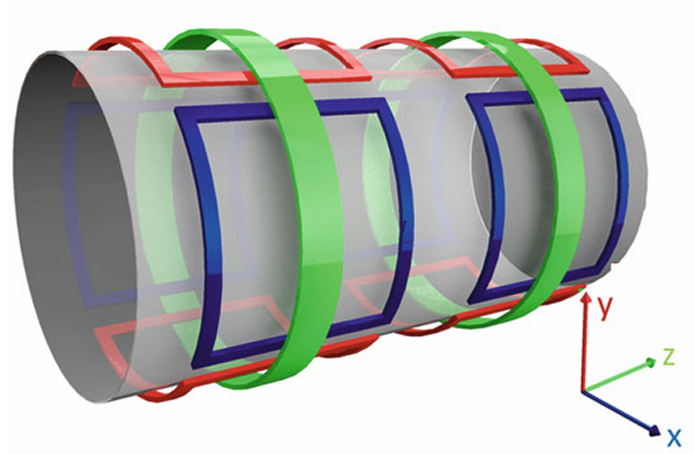
\includegraphics[scale=0.4]{/nfs/homes/sdreyer/Digit-Classification-Pytorch/tudothesis-main/content/abbildungen/Anordnung Gradientenspulen.png}
  \caption{Anordnung der Gradientenspulen.\cite{Schlegel}}
  \label{fig:an Grad}
\end{figure}
Durch das schalten der Gradienten kommt es zur Überlagerung mit dem Magnetfeld, wodurch die Codierung des Bildes möglich ist.
Der Gradient in z-Richtung wird für die Einstellung der Schichtdicke verwendet. 
Zur Frequenzcodierung wird der Gradient $G_x$ geschaltet, wodurch sich die Lamorfrequenzen entlang des Gradienten verschieben.
Mittels des Gradienten $G_y$ werden die Spins in ihrer Phase verschoben.
Durch die Verschiebung der Frequenz und Phase ist die Ortscodierung möglich und die Aufnahme eines Bildes im k-Raum.
Durch die Fouriertransformation werden die Informationen in den Ortsraum transformiert.
Dadurch liefert die MRT Bilder in Schichten, die anschließend zu einem 3D-Bild zusammengesetzt und analysiert werden.~\cite{pabst2013}

\section{Maschinelles Lernen}
Künstliche Intelligenz (KI) bezeichnet die Modellierung menschlicher Intelligenz durch Maschinen. 
Das Maschinelle Lernen (ML) ist ein Teilbereich der Künstlichen Intelligenz. Deep Learning stellt 
wiederum einen Teilbereich des maschinellen Lernens da. Das Deep learning beinhaltet das trainieren mehrschichtiger Neuronaler Netzwerke mit großen Datensätzen.
Die verschieden Teilbereiche der Künstliche Intelligenz werden in der Abbildung \ref{fig:KI} dargestellt.
Durch die Verwendung von Daten ist es den Algorithmen beim 
Maschinellem Lernen möglich aus diesen zu lernen und sich zu verbessern, ohne das die Algorithmen dem Problem entsprechend programmiert werden müssen.~\cite{kleesiek2020}
Somit findet das Maschinelle Lernen Anwendung in der Identifizierung und Klassifikation von Objekten, Analyse, Vorhersagen, 
Sprachverarbeitung, Informationsbeschaffung und in weiteren Bereiche.~\cite{shinde2018}
\begin{figure}[H]
  \centering
  \includegraphics[scale=0.4]{/nfs/homes/sdreyer/Digit-Classification-Pytorch/tudothesis-main/content/abbildungen/Künstliche Intelligenzpng.png}
  \caption{Künstliche Intelligenz und ihre Teilbereiche.~\cite{kleesiek2020}}
  \label{fig:KI}
\end{figure}
Das Lernen lässt sich unterscheiden in überwachtes Lernen (Supervised Learning) und unüberwachtes Lernen (Unsupervised Learning).
Beim überwachten Lernen, sind die Eingabedaten gelabelt, sodass das Netzwerk anhand dessen lernt, indem es den Ausgabewert mit dem bekannten Zielwert 
vergleicht und das Netzwerk dementsprechend anpasst.
Beim unüberwachten Lernen erkennt der Algorithmus Muster und Strukturen in den Eingabedaten, ohne das Eingabedaten gelabelt sind.~\cite{kleesiek2020}
\subsection{Neuronales Netzwerk}
Das Neurale Netzwerk ist aufgebaut aus drei Schichten: 
Die Eingabeschicht (Input Layer), versteckten Schichten (Hidden Layers) und die Ausgabe Schicht (Output Layer).
Die Input Layer nimmt die Daten auf und den Neuronen wird ein Wert zugeordnet.
Bei den Hidden Layers handelt es sich um mehrere Schichten, die sich zwischen der Eingabe- und Ausgabeschicht befinden.
In diesen werden die Eingabedaten verarbeitet und die Ergebnisse an die Ausgabeschicht weitergegeben.
Die Neuronen der versteckten Schichten erhalten dabei keine Daten von Außerhalb und geben keine raus. 
Der Aufbau eines Neuronalen Netzwerkes wird in der Abbildung \ref{fig:NN} dargestellt.
\begin{figure}[H]
  \centering
  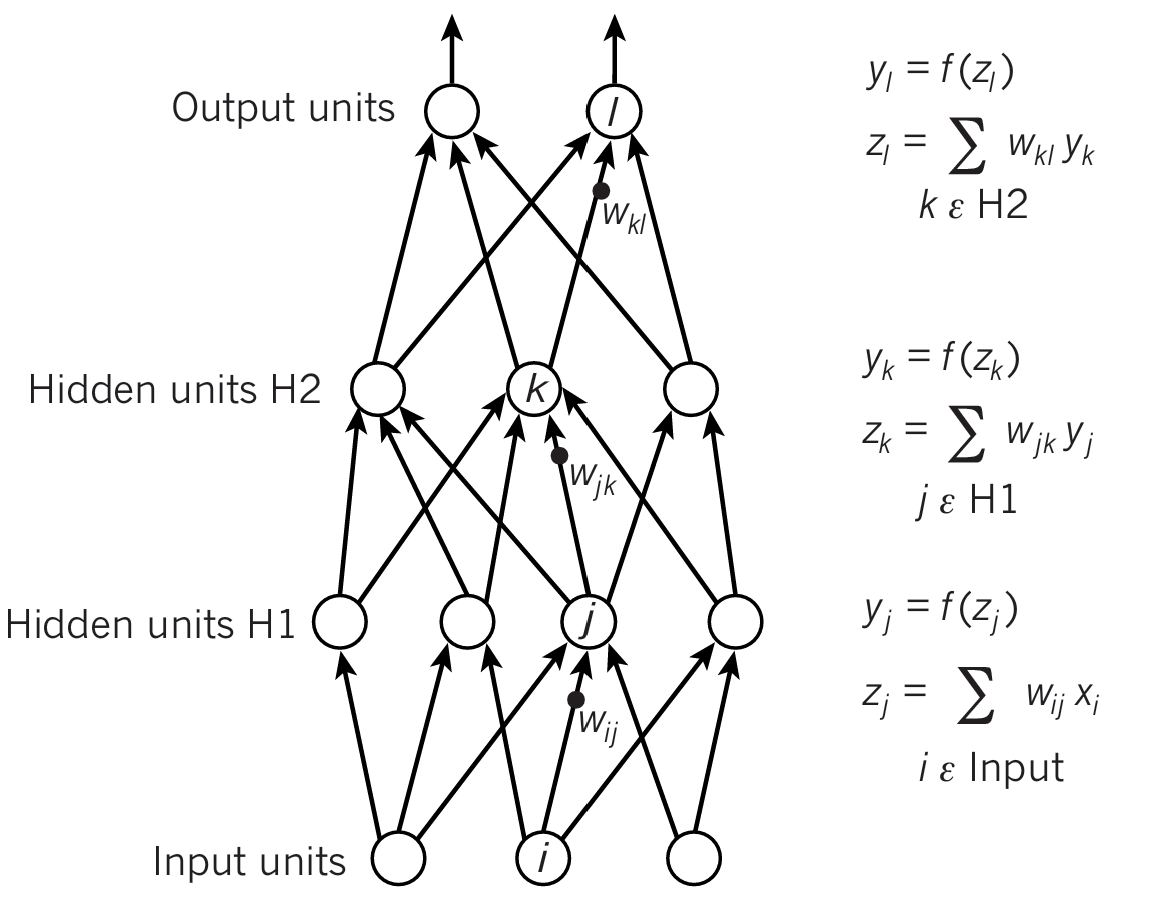
\includegraphics[scale=0.4]{/nfs/homes/sdreyer/Digit-Classification-Pytorch/tudothesis-main/content/abbildungen/Aufbau NN.png}
  \caption{Aufbau eines Fully Connected Neural Network.~\cite{lecun2015deep}}
  \label{fig:NN}
\end{figure}
Die nachfolgende Beschreibung bezieht sich auf den Aufbau dieses Netzwerkes.
Jedes Neuron ist dabei mit jedem aus der Vorherigen Schicht verbunden durch eine Gewichtung $w_{ij}$.
Die Aktivierung eines Neurons wird mittels einer Aktivierungsfunktion $f_\text{act}$ berechnet. In dieser fließt unter anderem die Gewichtung, 
der Eingabe Wert $x_i$ sowie ein Bias-Wert $b_j$ mit ein.
Der Output des Neurons j lässt sich somit über 
\begin{equation}
    y_j = f_\text{act}\left(\sum_{i}^{n} w_{ij}x_i + b_j\right)
\end{equation}
berechnen.
Dieser Ausgabewert $y_j$ wird an die Neuronen in der nächsten Schicht weitergegeben.
Die meist verwendetet Aktivierungsfunktionen sind die Sigmoidfunktion, Rectifier-Funktion (ReLU-Funktion) und der hyperbolische Tangens.
Wird der Schwellenwert bei diesen Funktionen nicht erreicht, wird der Wert des Neurons nicht an die nächste Schicht weitergegeben.
Das Neuron wird inaktiv.
Bei der ReLU-Funktion beträgt der Schwellenwert 0, sodass die Ausgangswerte nur im positiven Bereich liegen.
Die Sigmoidfunktion gibt einen Ausgabewert zwischen 0 und 1, da diese Funktion auf diesen Wertebereich normalisiert ist.
Beim verwenden des hyperbolischen Tangens, befindet sich der Wertebereich zwischen -1 und +1.~\cite{datascience}

\subsection{Convolutional Neural Network}\label{sec:NN}
Für die Verarbeitung von Bildern eignet sich das Fully Connected Neural Network, wie es in \ref{fig:NN} dargestellt ist, nicht, da jedes Pixel ein Eingabewert darstellt.
Aufgrund der Verbindung jedes Neurons aus der vorherigen Schicht, kommt es zu einer großen Anzahl an Verbindungen.
Durch die große Anzahl an Rechenoperationen ist das Training des Netzwerkes ineffizient.
Aus diesem Grund und zur Nutzung der räumlichen Korrelation der Pixel wird für die Verarbeitung von Bildern das Convolutional Neural Network (CNN) verwendet.
Bei diesem sind die Neuronen in drei Dimensionen angeordnet.
Diese sind die zwei räumlichen Dimensionen Breite und Höhe und die dritte Dimension bildet die Anzahl an Kanälen.
Der Beispielhafte Aufbau eines CNN in seiner Standardform wird in der Abbildung \ref{fig:CNN} dargestellt.
Dabei ist das Netzwerk aufgebaut aus Faltungschichten (Convolutional Layers), Pooling Layers und einer Fully-Connected Layer (FC-Layer).
Zwischen den Schichten wird, wie bei den Neuronalen Netzwerken eine Aktivierungfunktion verwendet.~\cite{OShea} 
\begin{figure}[H]
  \centering
  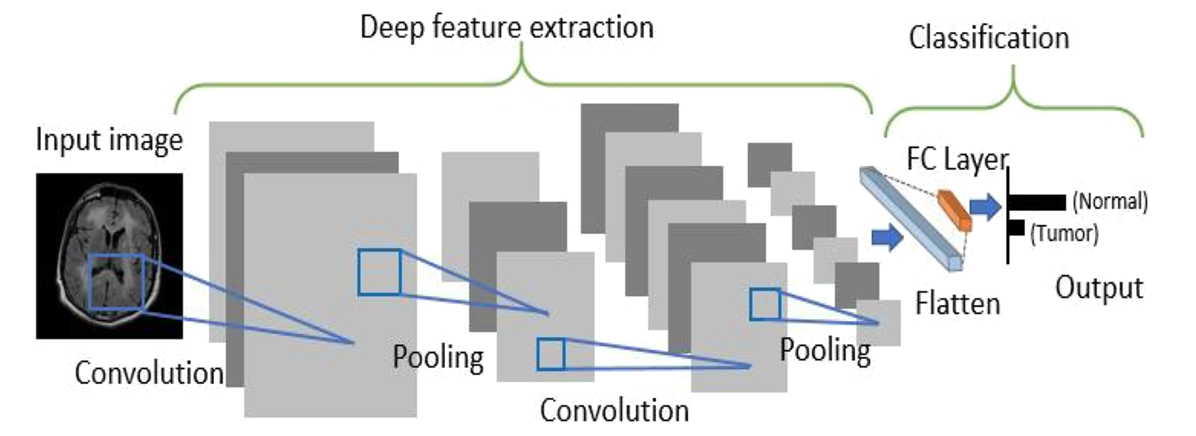
\includegraphics[scale=0.3]{/nfs/homes/sdreyer/Digit-Classification-Pytorch/tudothesis-main/content/abbildungen/CNN.png}
  \caption{Aufbau eines Convolutional Neural Network.~\cite{Mohammed2024}}
  \label{fig:CNN}
\end{figure}
Bei der Convolutional Layer, wird ein Filter (Kernel) verwendet, welcher schrittweise über das gesamte Input Bild gelegt wird.
Dieser besitzt meist eine typische Größe von $3 \times 3$, $5 \times 5$ oder $ 7 \times 7$.  
Aus dem Kernel und dem Neuron wird das Skalarprodukt berechnet, aus dem eine Feature-Map erstellt wird. 
Diese Feature-Map beinhaltet die wichtigsten Strukturen und Merkmale.~\cite{Yamashita2018}
Der Ausgabewert der Feature-Map an der Position (i,j) ergibt sich durch die Faltung
\begin{equation}
  S(i,j) = (K * I)(i, j) = \sum_m \sum_n I(i + m, j + n) \cdot K(m,n).
\end{equation}
Dabei beschreibt $I$ das Eingabebild und $K$ den Kernel.~\cite{Goodfellow-et-al-2016}
Damit der Filter auch den Rand des Bildes mit dem Zentrum überlappen kann, wird das sogenannte Padding angewendet.
Beim Zero-padding, werden am Rand des Bildes Nullen hinzugefügt. Dadurch bleibt die räumliche Dimension erhalten.
Als Stride wird der Abstand zwischen zwei Positionen des Kernels beschrieben. Am häufigsten wird ein stride von 1 gewählt. 
Das bedeutet, dass sich nach jeder Berechnung des Skalarproduktes der Kernel um eine Position verschiebt.
\begin{figure}[H]
  \centering
  \begin{subfigure}[b]{0.3\textwidth}
    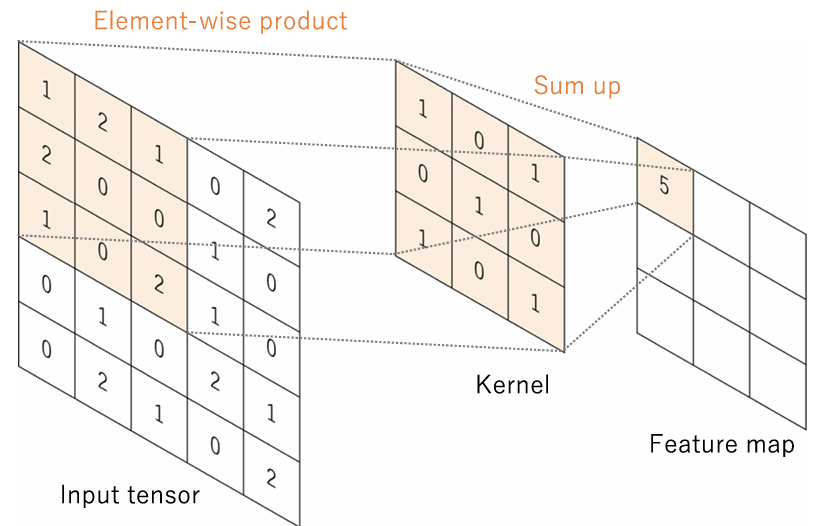
\includegraphics[width=\textwidth]{/nfs/homes/sdreyer/Digit-Classification-Pytorch/tudothesis-main/content/abbildungen/kernel a.png}
    %\caption{}
    \label{}
  \end{subfigure}
  \hfill
  \begin{subfigure}[b]{0.3\textwidth}
    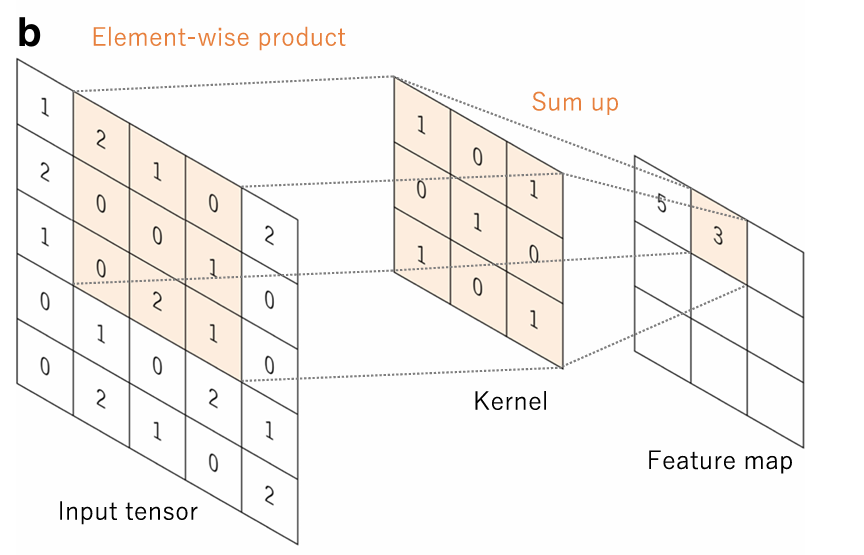
\includegraphics[width=\textwidth]{/nfs/homes/sdreyer/Digit-Classification-Pytorch/tudothesis-main/content/abbildungen/kernel b.png}
    %\caption{}
    \label{}
  \end{subfigure}
  \hfill
  \begin{subfigure}[b]{0.3\textwidth}
    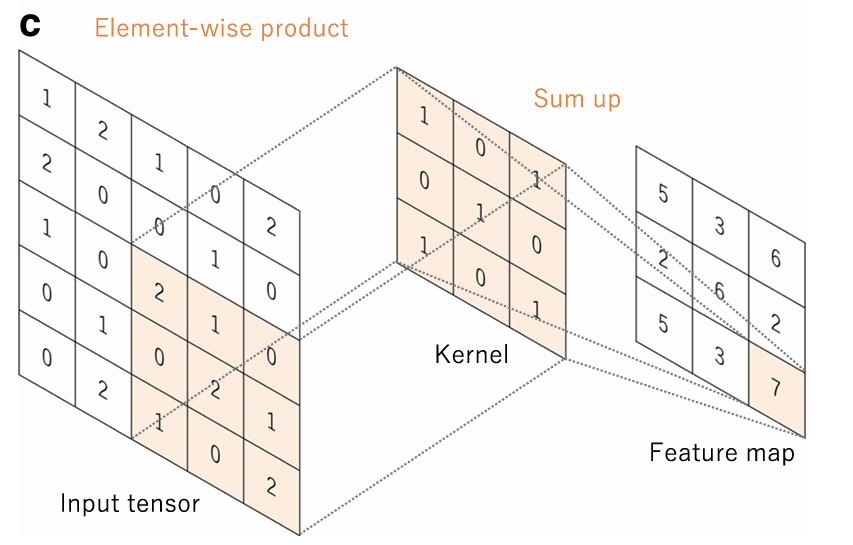
\includegraphics[width=\textwidth]{/nfs/homes/sdreyer/Digit-Classification-Pytorch/tudothesis-main/content/abbildungen/kernel c.png}
    %\caption{}
    \label{}
  \end{subfigure}
  \caption{Ein Beispiel der Convolutional layer mit der Verwendung eines Kernels der Größe $3 \times 3$.~\cite{Yamashita2018}}
  \label{fig:kernel}
\end{figure}
Die Pooling-Layer reduziert die räumliche Dimension. Infolge dessen kommt es auch zur Reduktion der Parameter.~\cite{datascience}
Dafür wird das sogenannte Max-Pooling verwendet. Dabei wird ein Filter der Größe $2 \times 2$ verwendet, der wie der Kernel, schrittweise über die Feature-Map gelegt wird.
Für jeden Ausschnitt wird der größte Wert verwendet. Der Rest der Werte wird nicht weiter verwendet.~\cite{Yamashita2018}\\
%Dies wird in der Abbildung 
%\begin{figure}[H]
%  \centering
%  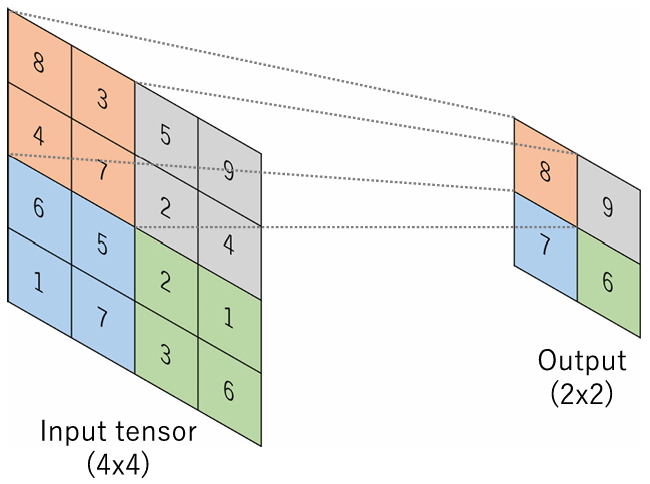
\includegraphics[scale=0.4]{/nfs/homes/sdreyer/Digit-Classification-Pytorch/tudothesis-main/content/abbildungen/max_pooling.png}
%  \caption{Eine Beispielhafte Anwendung von Max-Pooling mit einem $2 \times 2$ Filter.~\cite{Yamashita2018}}
%  \label{fig:CNN}
%\end{figure}
Die FC-Layer berechnet am Ende die Aktivierung und bestimmt einen Ausgangswert für die Klassifizierung.
Sie entspricht damit der Art von Output-Layer, die in Kapitel \ref{sec:NN} beschrieben wurde.

\subsection{Training eines Netzwerkes}
Beim Training der Netzwerke, werden die Gewichtungen zwischen den Neuronen schrittweise angepasst. 
Zu Beginn wird den Gewichtungen ein Zufälliger Wert zu geschrieben.
Beim Training, wird zur Anpassung der Gewichtungen der Backpropagation-Algorithmus verwendet.
Dabei wird die sogenannte Verlustfunktion (Loss Function) angewendet, welche den Fehler zwischen dem Ausgabewert des Netzwerkes und den bekannten Zielwert berechnet.
Ziel des Training ist es das Minimum der Verlustfunktion zu ermitteln, indem die Parameter angepasst werden.~\cite{datascience}
Häufige Verlustfunktionen sind beispielsweise der Mean Squared Error (MSE)
\begin{equation}
  \text{MSE}  =  \frac{1}{n} \sum_{i=1}^{n} (y_i - \hat{y}_i)^2
\end{equation}
oder die Binary Cross-Entropie für die Klassifikation zwischen zwei Klassen  
\begin{equation}
\text{CE} = -\frac{1}{n} \sum_{i=1}^{n} \left( y_i \cdot \log(\hat{y}_i) + (1 - y_i) \cdot \log(1 - \hat{y}_i) \right).
\label{eq:BCE}
\end{equation}
Dabei beschreibt $n$ die Anzahl an Training samples, $y_i$ den Zielwert und $\hat{y}_i$ den berechneten Ausgabewert.
Durch den Backpropagation-Algorithmus wird die partielle Ableitung der Verlustfunktion mittels der Kettenregel berechnet.
Da der Gradient in die Richtung des größten Anstiegs zeigt, erfolgt die Anpassung der Gewichte in die entgegengesetzte Richtung. 
Eine positive Ableitung führt somit zur Verringerung, eine negative zur Erhöhung der Gewichtung.~\cite{neuralnet}
Der Optimizer passt auf Grundlage des Gradienten die Parameter an und sorgt dafür, dass diese im Netzwerk aktualisiert werden.
Zu den häufigsten verwendeten Optimizer sind der SGD, RMSprop und Adam.
Zusätzlich wird beim Training eine Validierung durchgeführt um die Hyperparameter zu optimieren. 
Hierzu wird der Datensatz aufgeteilt, in Training- und Validierungsdaten, wobei die Validierungsdaten nicht zur Aktualisierung 
der Gewichtungen verwendet werden.~\cite{Yamashita2018}
Als Hyperparameter werden die Parameter bezeichnet, die zu Beginn des Trainings manuell festgelegt werden.
Zu diesen gehört unter anderem die Lernrate, die Batch-Größe, die Anzahl an Schichten und Neuronen, die Anzahl an Trainingsdurchläufen (Epochen)
und die Verlustfunktion.
Die Batch-Größe gibt an, wie viele Trainingsdaten pro Trainingsschritt verwendet werden.~\cite{datascience} 
Die Lernrate legt fest, wie stark die Gewichte bei jedem Trainingsschritt angepasst werden.~\cite{Mohammed2024} 
Um Overfitting zu vermeiden, wird der sogenannte Dropout als weiterer Hyperparameter eingebaut.
Der Dropout schaltet während des Trainings zufällige Neuronen aus.
Dadurch stützt sich das Netzwerk nicht auf Spezifische Neuronen und das Netzwerk wird robuster. ~\cite{Yamashita2018}.

Wenn ein Modell neben den relevanten Mustern auch die irrelevante Störungen lernt, die nur in den Trainingsdaten enthalten sind, gilt es als zu stark an den Trainingsdaten angepasst.
Bei der Anwendung des Netzwerkes auf einen unabhängigen Datensatz, verschlechtert sich die Leistung deutlich. 
Dieses Verhalten wird dann als Overfitting bezeichnet.
Um zu überprüfen, ob das Modell überangepasst ist, wird der Validierungsverlust (Validation Loss) während des Trainings mitbeobachtet.
Wenn der validation loss ansteigt, der Trainings Verlust jedoch kontinuierlich sinkt, ist dies ein Zeichen, dass das Netzwerk überangepasst wird.~\cite{Yamashita2018}
Dies wird in der Abbildung \ref{fig:overfitting} graphisch dargestellt.
\begin{figure}[H]
  \centering
  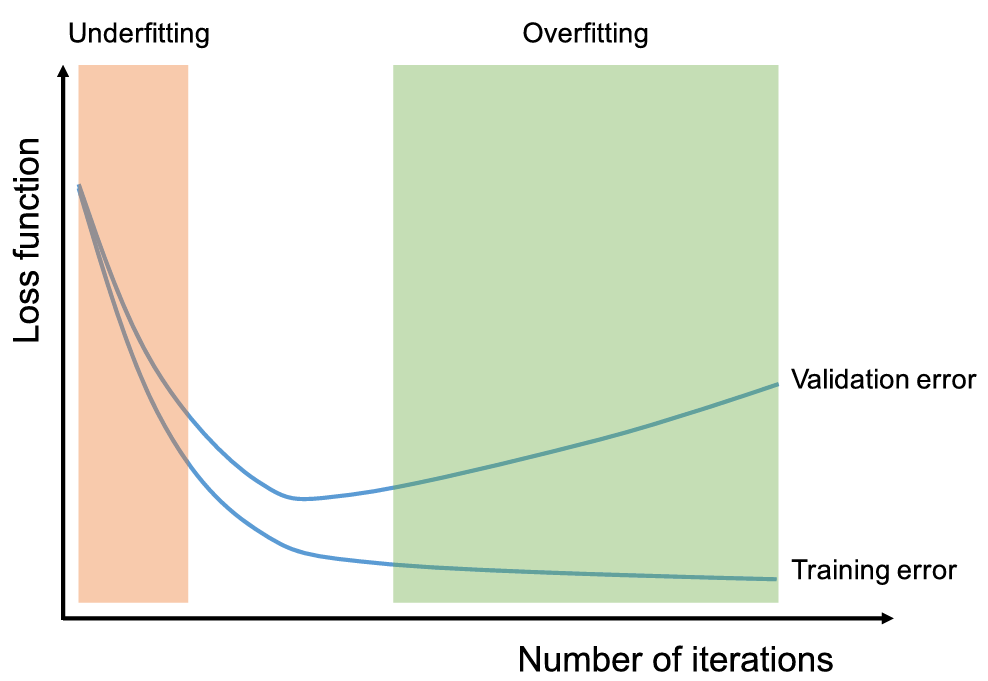
\includegraphics[scale=0.23]{/nfs/homes/sdreyer/Digit-Classification-Pytorch/tudothesis-main/content/abbildungen/Overfitting.png}
  \caption{Überprüfung auf Overfitting durch das Kontrollieren des Trainings und validation loss.~\cite{Yamashita2018}}
  \label{fig:overfitting}
\end{figure}
%Möglichkeiten um Overfitting zu vermeiden sind zum einen, das mehr Daten verwendet werden. 
%Zudem kann ein Dropout implementiert werden. Der Dropout schaltet während des Trainings zufällige Neuronen aus.
%Dadurch stützt sich das Netzwerk nicht auf Spezifische Neuronen 
\chapter{Methodik}

\section{Datensatz}
Für diese Arbeit wurde Datensatz "Brain Tumor MRI Dataset", welcher auf Kaggle veröffentlicht wurde, verwendet.~\cite{msoud_nickparvar_2021}
Dieser beinhaltet die vier Klassen: no Tumor, Glioma, Meningioma und Pituitary.
In dieser Arbeit wird die Klasse Pituitary nicht betrachtet.
Aufgeteilt ist der Datensatz in Trainingsdaten und Testdaten.
Die Anzahl der verwendet samples sind in der Tabelle \ref{tab:daten} dargestellt. 
\begin{table}[htbp]
    \centering
    \begin{tabular}{l c r}
        \hline
        Klasse      & Training samples & Test samples \\
        \hline
        no Tumor    &    1595          & 405 \\
        Glioma      &    1321          & 300 \\
        Meningioma  &    1339          & 306 \\
        \hline
  \end{tabular}
  \caption{Anzahl der verwendeten Training sample und Test samples.}
  \label{tab:daten}
\end{table}
Im Folgenden wurde zwei unterschiedliche Klassifikationen durchgeführt.
Zu nächst wurde das CNN trainiert, dass es zwischen der Klasse no Tumor und Tumor unterscheidet. Für die Klasse Tumor
wurde die samples der Glioma und Meningioma Klasse zusammengefasst.
Die zweite Klassifikation besteht darin zwischen, dass das CNN unterscheidet, um welche Tumorart es sich handelt.
Dementsprechend wurde ausschließlich die Klasse Glioma und Meningioma betrachtet.
Dabei wird die Meningioma Klasse als Positiv  und die Glioma Klasse als negativ definiert.\\


Die verwendeten MRT Bilder werden zu beginn auf die Größe $224 \times 224$ Pixel skaliert, aufgrund dessen, dass die Bilder nicht alle die 
gleiche Größe besitzen.
Zudem wurden die Bilder in ein Array umgewandelt und Normiert auf die Werte [0,1].\\

Für das Training des Netzwerkes werden die Training samples aufgeteilt. $\qty{80}{\%}$ der Daten, werden zum trainieren des Netzwerkes 
verwendet und $\qty{20}{\%}$ zur Validierung.
Die Aufteilung der Bilder bleibt für jeden Durchgang des Trainierens gleich.

\section{CNN + Metriken}

Das verwendete CNN besteht aus vier Convolutional Layers. Als Aktivierungsfunktion wurde die ReLU-Funktion verwendet.
Zudem wird ein $3 \times 3$ Kernel und Max-Pooling einer Größe von $2 \times 2$ eingesetzt. 
Jede Convolutional Schicht beinhalt Stride und Padding mit dem Wert 1.
Da die MRT Graustufenbilder sind, besitzt das Input Bild einen Kanal von eins. 
In der ersten Schicht werden 32 Filter verwendet.
Die Anzahl erhöht sich in jeder Schicht um den Faktor zwei.
Somit werden in der letzten Convolutional Schicht 128 Filter verwendet.
In der FC-Layer wurde ein Dropout implementiert.\\

Zur Beurteilung der Leistungsfähigkeit, wird für jede Klassifikation die Accuracy, Sensitivity und Specificity berechnet.
Die Accuracy wird über
\begin{equation}
  Accuracy = \frac{TP + TN}{TP + TN + FP + FN}
\end{equation}
berechnet.
Die Sensitivity beschreibt wie viele Krankheitsfälle korrekt erkannt wurden. Dies lässt sich über
\begin{equation}
  Sensitivity = \frac{TP}{TP + FN}
\end{equation}
berechnen.
Die Specificity wird über die Formel
\begin{equation}
  Specificity = \frac{TN}{TN + FP}
\end{equation}
ermittelt und gibt die Richtig Fälle an, bei dem sich um keine Krankheit handelt.%~\cite{west2020sensitivity}

\section{Hyperparameter}



\section{Trainingssamples reduzieren}


\section{Augmentierung}


\section{Reduzierung einer Sample Klasse}

\chapter{Ergebnisse}
\section{Klassifizierung zwischen Tumor und no Tumor}
\subsection{Hyperparameter}
Um die Hyperparameter zu ermitteln, werden die fünf Trainingsdurchläufen (Runs) mit den niedrigsten Validation Loss betrachtet.
In der Abbildung \ref{fig:val_loss notu-tu} wird der Verlauf des validation loss dargestellt.
\begin{figure}[H]
  \centering
  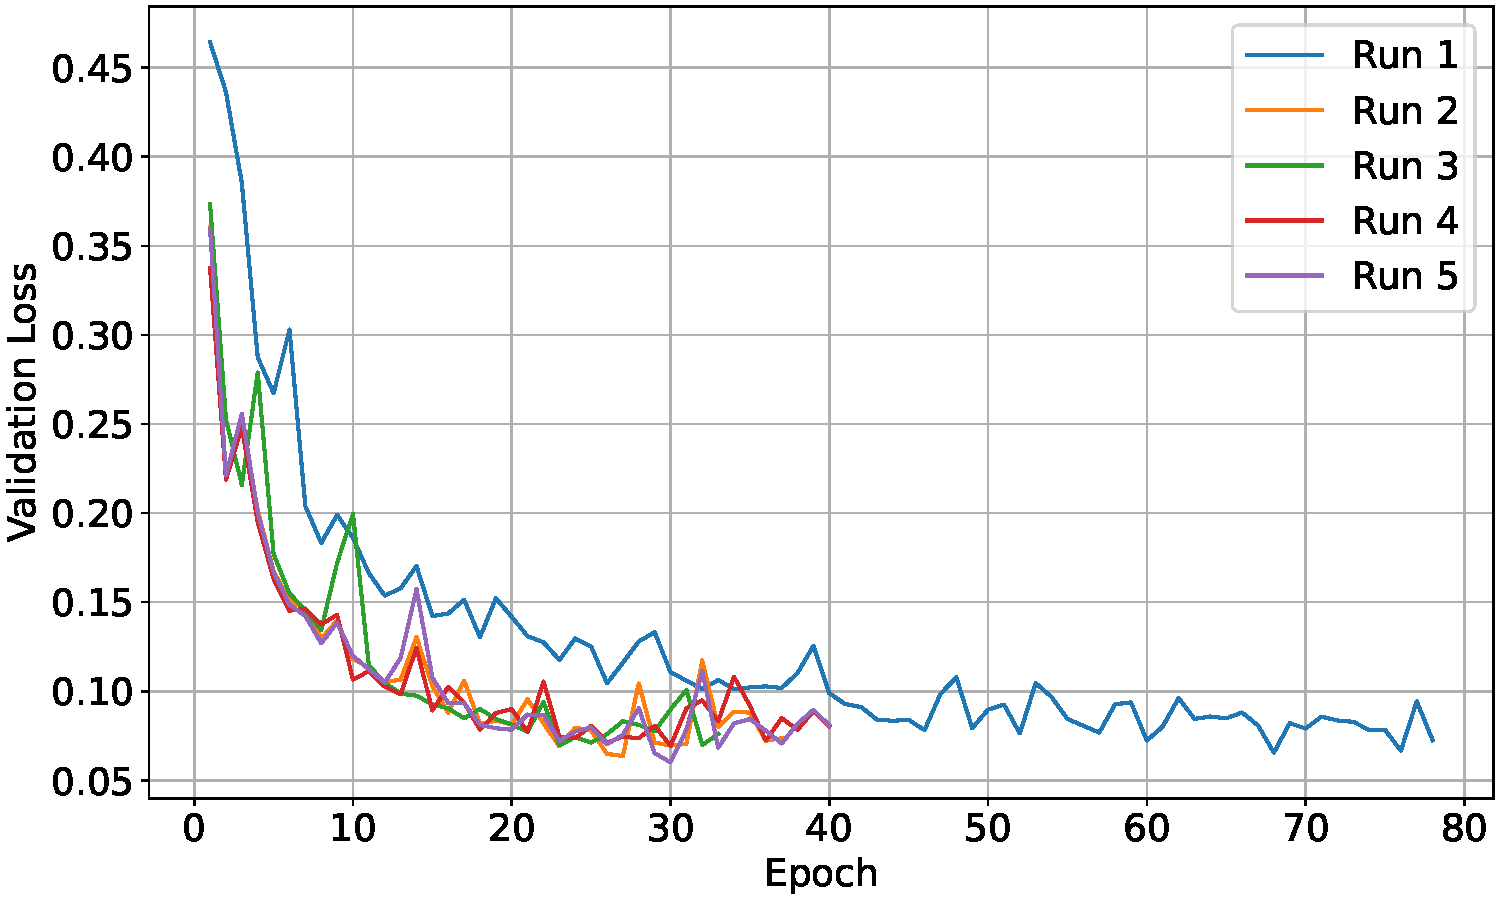
\includegraphics[scale=0.4]{plots/Val_loss_noTu_Tu.pdf}
  \caption{Verlauf des validation loss bei der Verwendung verschiedener Hyperparameter.}
  \label{fig:val_loss notu-tu}
\end{figure}
\vspace{-2em}
Die verwendeten Werte der Hyperparameter für diese fünf Runs, sowie die aufgenommene Accuracy, Sensitivity und Specificity der Validierungsdaten,
werden in der Tabelle \ref{tab:hyperp notu-tu} aufgezeigt.
\begin{table}[H]
    \centering
    \resizebox{\textwidth}{!}{%
        \begin{tabular}{cccccccc}
            \toprule
            Runs & Batch Größe & Lernrate & Dropout & validation loss & Accuracy/$\%$ & Sensitivity & Specificity \\
            \midrule
            1 & 128 & 0.005  & 0.55 & 0.072539 & 97.53231 & 0.97967 & 0.96774 \\
            2 & 128 & 0.0005 & 0.5  & 0.073672 & 98.00235 & 0.98706 & 0.96774 \\
            3 & 16  & 0.0001 & 0.5  & 0.076007 & 97.88484 & 0.97597 & 0.98387 \\
            4 & 128 & 0.0005 & 0.4  & 0.080399 & 97.76733 & 0.97782 & 0.97742 \\
            5 & 128 & 0.0005 & 0.5  & 0.080853 & 97.64982 & 0.98706 & 0.95806 \\
            \bottomrule
        \end{tabular}
    }
  \caption{Die fünf Runs mit dem niedrigsten validation loss sowie deren verwendete Hyperparameter und aufgezeichnete Metriken.}
  \label{tab:hyperp notu-tu}
\end{table}
Die Werte der Accuracy, Sensitivity und Specificity liegen dicht bei einander und schwanken nur geringfügig.
Da die Ergebnisse der Validierung konstant sind, werden für die weiteren Trainingsdurchläufen die Hyperparameter des Runs 1 verwendet. 

\subsection{Reduzierung der Trainingsdaten}

Das Netzwerk wurde mit unterschiedlichen Datensatzgrößen trainiert und auf einen Testdatensatz angewendet, bei dem die Accuracy, Sensitivity und Specificity berechnet wurde.
Da beobachtet wurde, dass die Werte der Metriken bei 2723 gesunken sind, wurde zusätzlich das Netzwerk mit 2553, 2893 und 3234 
Training samples trainiert.
Die Mittelwerte und Standardabweichung der Metriken wurden in Abhängigkeit von den Training samples dargestellt.
Diese Ergebnisse sind in Abbildung \ref{fig:reduzierung_trainingsdaten} sowie Tabelle \ref{tab:reduzierung_trainingsdaten} zusammengefasst.
Es ist zu erkennen, dass die drei Metriken einen ähnlichen Verlauf aufweisen.
Die niedrigsten Werte werden bei 340 Training samples aufgenommen und steigen dann kontinuierlich mit der sample Anzahl an.
Ab 2042 verwendete samples zeigen die Werte der Accuracy, Sensitivity und Specificity nur noch geringe Änderungen  .
Dabei schwankt die Accuracy im Bereich zwischen 2042 und 3404 Training samples zwischen $\qty{93.1157}{\%}$ und $\qty{96.2611}{\%}$. 
Die Werte der Sensitivity variieren in diesem Bereich zwischen 0,9147 und 0,9462 und die der Specificity um \SI{0,9741}{} und \SI{0,9872}{}.
\begin{figure}[H]
  \centering
  \begin{subfigure}[b]{0.48\textwidth}
    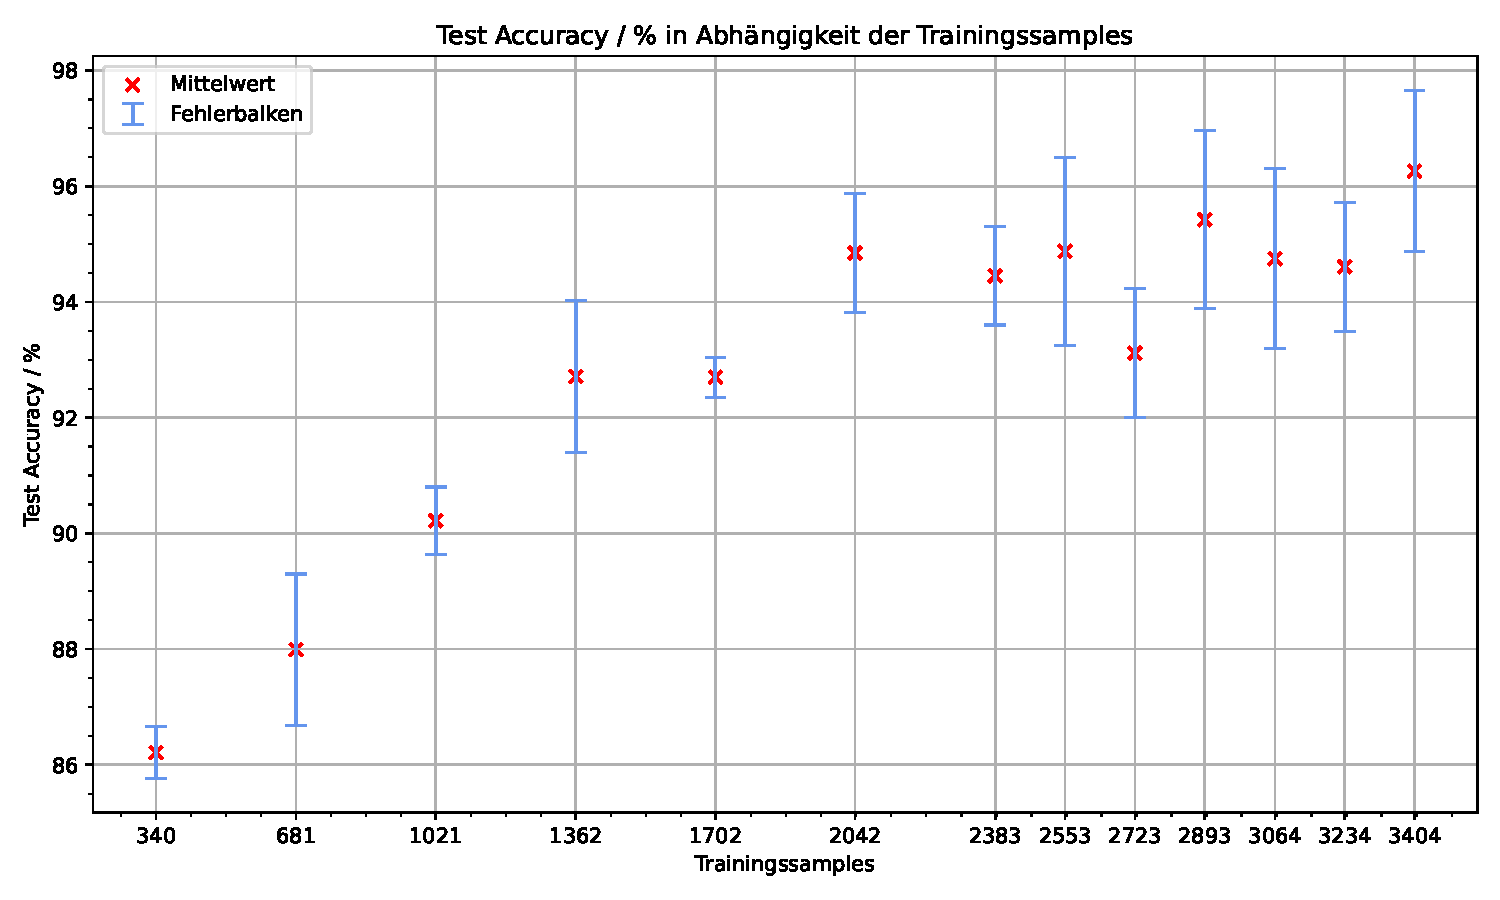
\includegraphics[width=\textwidth]{plots/2-Messungen-noTu-Tu_Accuracy_mean.pdf}
    \caption{Accuracy}
    \label{fig:reduzierung_accuracy}
  \end{subfigure}
  \begin{subfigure}[b]{0.48\textwidth}
    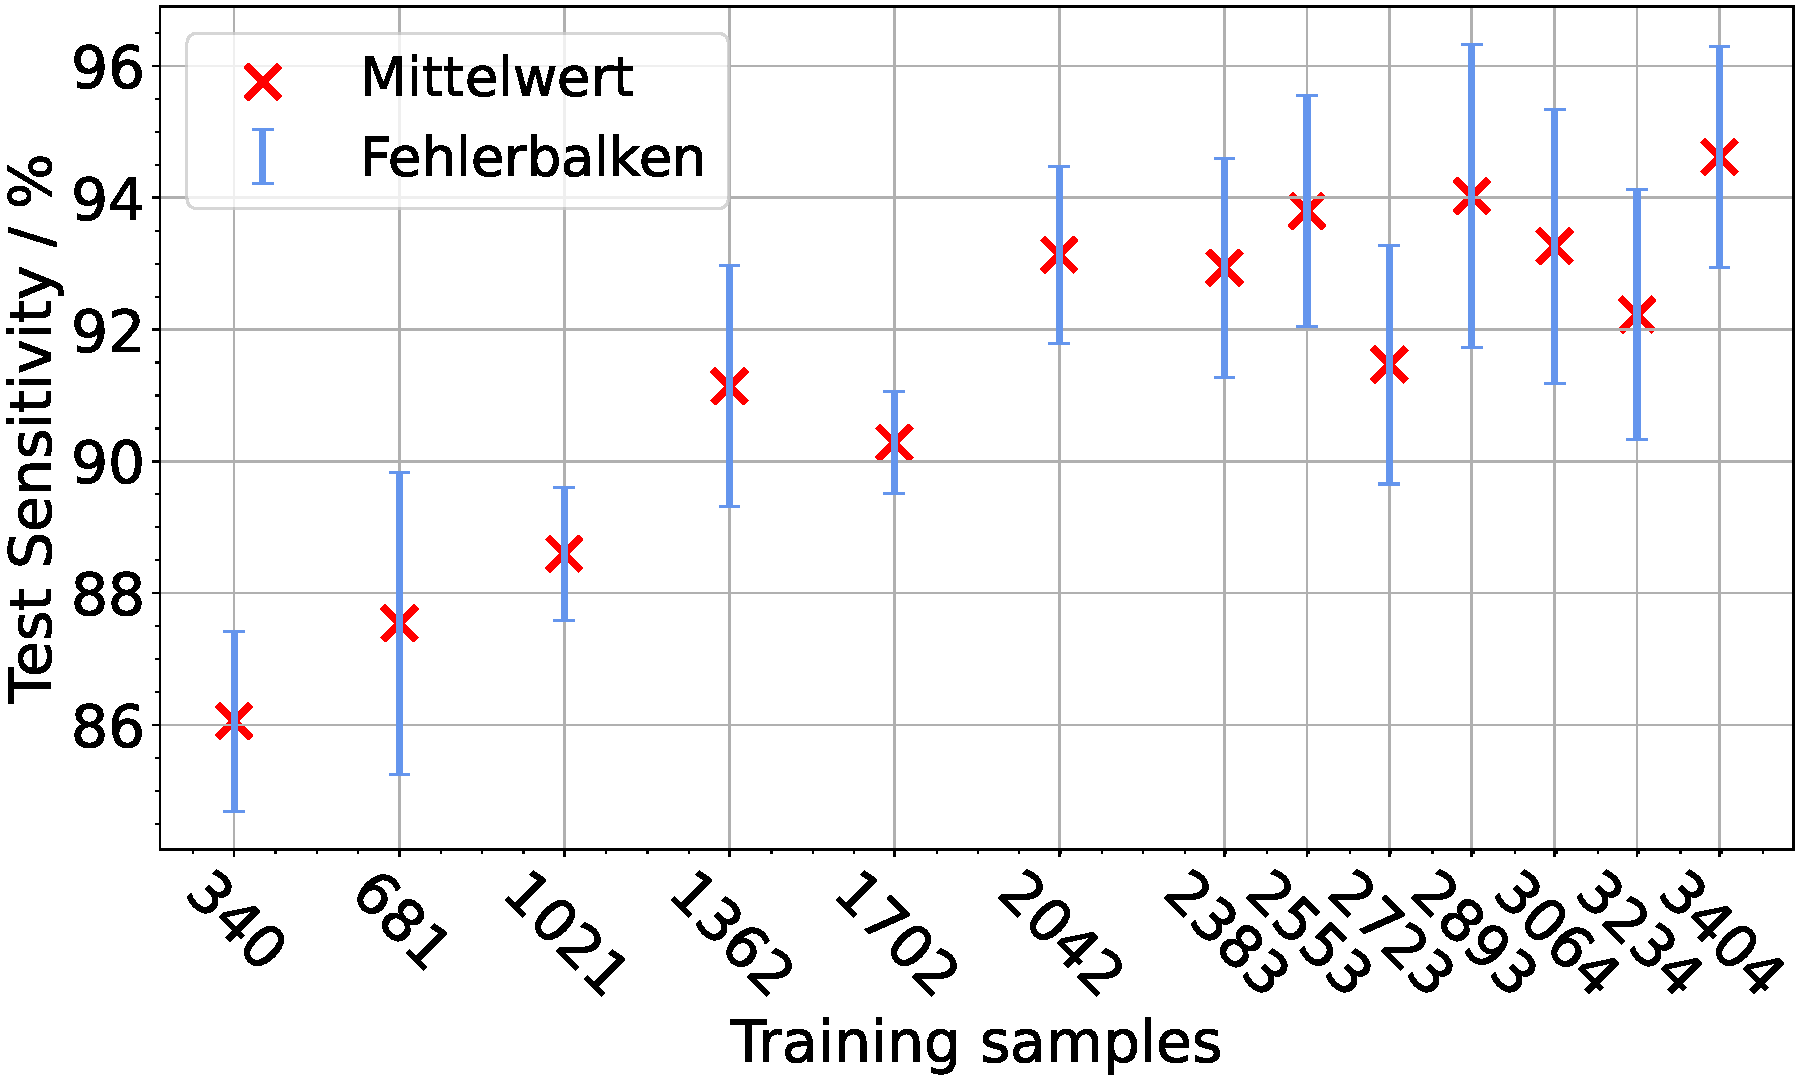
\includegraphics[width=\textwidth]{plots/2-Messungen-noTu-Tu_Sensitivity_mean.pdf}
    \caption{Sensitivity}
    \label{fig:reduzierung_sensitivity}
  \end{subfigure}
  \begin{subfigure}[b]{0.48\textwidth}
    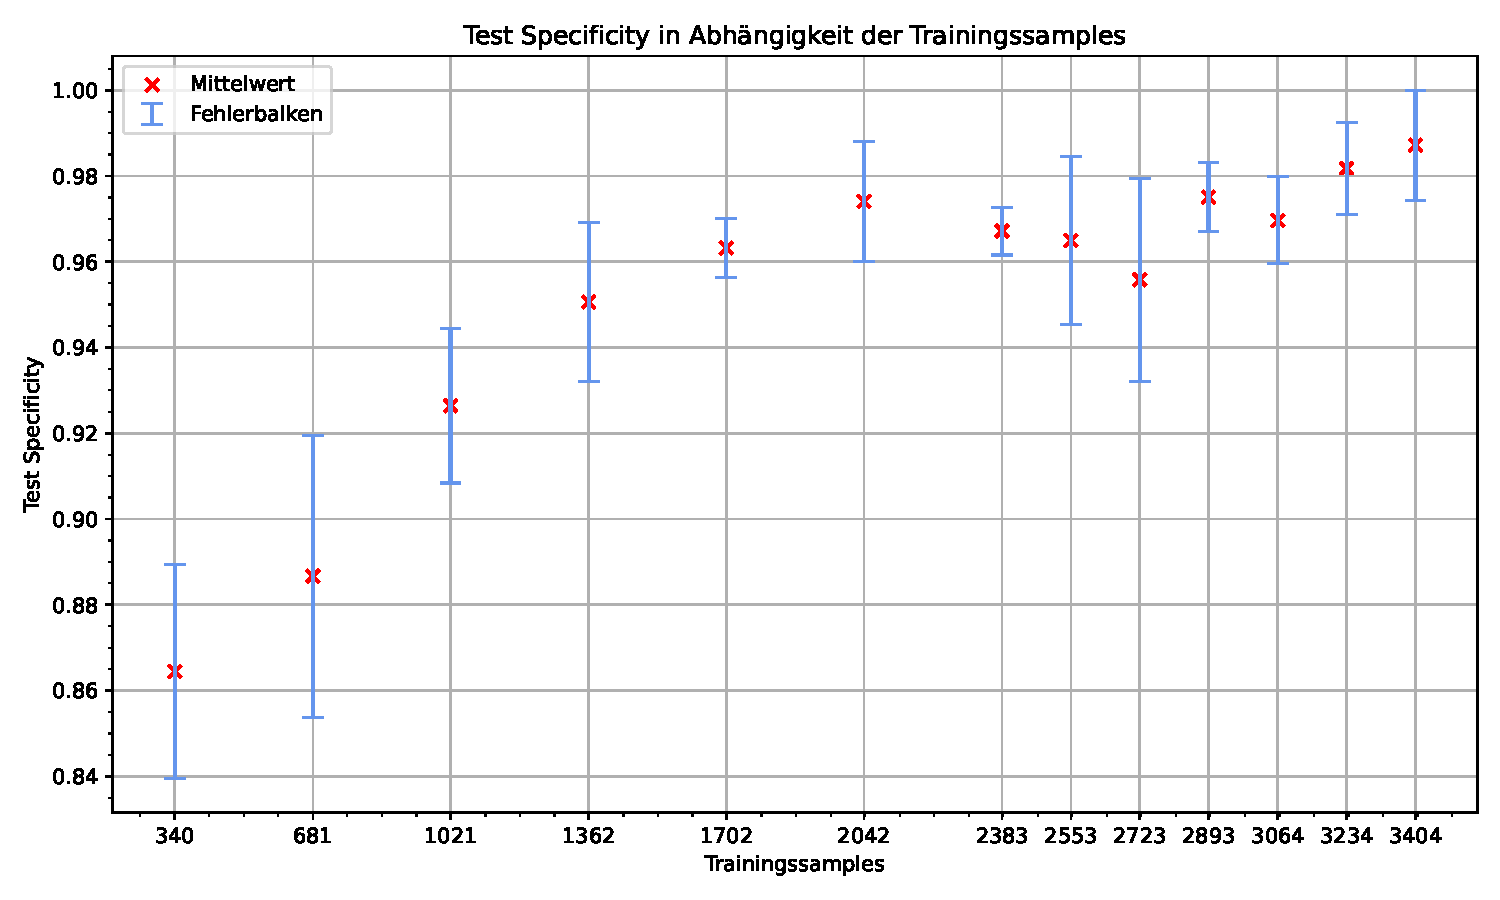
\includegraphics[width=\textwidth]{plots/2-Messungen-noTu-Tu_Specificity_mean.pdf}
    \caption{Specificity}
    \label{fig:reduzierung_specificity}
  \end{subfigure}
  \caption{Aufgenommene Metriken in Abhängigkeit der Verwendeten Trainingsdaten für die Klassifikation zwischen no Tumor und Tumor.}
  \label{fig:reduzierung_trainingsdaten}
\end{figure}
\begin{table}[H]
    \centering
    {\small
        \begin{tabular}{cccc}
            \toprule
            Training sample & Accuracy/\% & Sensitivity & Specificity\\
            \midrule
            340  & $86.2117 \pm 0.4428$ & $0.8606 \pm 0.0137 $ & $0.8644 \pm 0.0249$\\
            681  & $87.9921 \pm 1.3057$ & $0.8754 \pm 0.0229 $ & $0.8867 \pm 0.0329$\\
            1021 & $90.2176 \pm 0.5832$ & $0.8860 \pm 0.0101 $ & $0.9264 \pm 0.0180$\\
            1362 & $92.7102 \pm 1.3106$ & $0.9114 \pm 0.0183 $ & $0.9506 \pm 0.0186$\\
            1702 & $92.7003 \pm 0.3452$ & $0.9028 \pm 0.0078 $ & $0.9632 \pm 0.0068$\\
            2042 & $94.8467 \pm 1.0316$ & $0.9314 \pm 0.0134 $ & $0.9741 \pm 0.0140$\\
            2383 & $94.4510 \pm 0.8502$ & $0.9294 \pm 0.0166 $ & $0.9672 \pm 0.0056$\\
            2553 & $94.8764 \pm 1.6231$ & $0.9380 \pm 0.0175 $ & $0.9649 \pm 0.0196$\\
            2723 & $93.1157 \pm 1.1163$ & $0.9147 \pm 0.0181 $ & $0.9558 \pm 0.0237$\\
            2893 & $95.4204 \pm 1.5352$ & $0.9403 \pm 0.0230 $ & $0.9751 \pm 0.0080$\\
            3064 & $94.7478 \pm 1.5545$ & $0.9327 \pm 0.0208 $ & $0.9696 \pm 0.0102$\\
            3234 & $94.6093 \pm 1.1125$ & $0.9223 \pm 0.0190 $ & $0.9817 \pm 0.0108$\\
            3404 & $96.2611 \pm 1.3948$ & $0.9462 \pm 0.0167 $ & $0.9872 \pm 0.0128$\\ 
            \bottomrule
        \end{tabular}
    }
  \caption{Mittelwert und Standardabweichung der Metriken bei der Reduzierung der Training samples.}
  \label{tab:reduzierung_trainingsdaten}
\end{table}

\subsection{Augmentation}
Das Netzwerk wurde für verschiedene Datensatzgrößen trainiert, wobei beim Training Augmentation angewendet wurde.
Die Accuracy, Sensitivity und Specificity werden in Abhängigkeit der Training samples in Abbildung \ref{fig:augmentation_tu} abgebildet und
die dargestellten Werte werden in der Tabelle \ref{tab:augm-tunotu} aufgezeigt.
Von 340 bis 2042 Samples, steigt die Accuracy und die Specificity konstant an und geht anschließend in Plateau über.
Die Accuracy variieren innerhalb des Plateaus zwischen \SI{94.2532}{\percent} und \SI{96.4293}{\percent}. 
Die Specificity schwankt ab 2042 Training samples zwischen \SI{0.9234}{} und \SI{0.9475}{}.
Die Sensitivity steigt nur bis zu 1021 samples kontinuierlich an und bleibt bis zu 1702 Samples konstant bei ungefähr \SI{0,89}{}.
Danach steigt sie wieder an und schwankt, von 2042 bis 3404 Training samples, zwischen \SI{0.9234}{} und \SI{0.9475}{}. 
\begin{figure}[H]
  \centering
  \begin{subfigure}[b]{0.48\textwidth}
    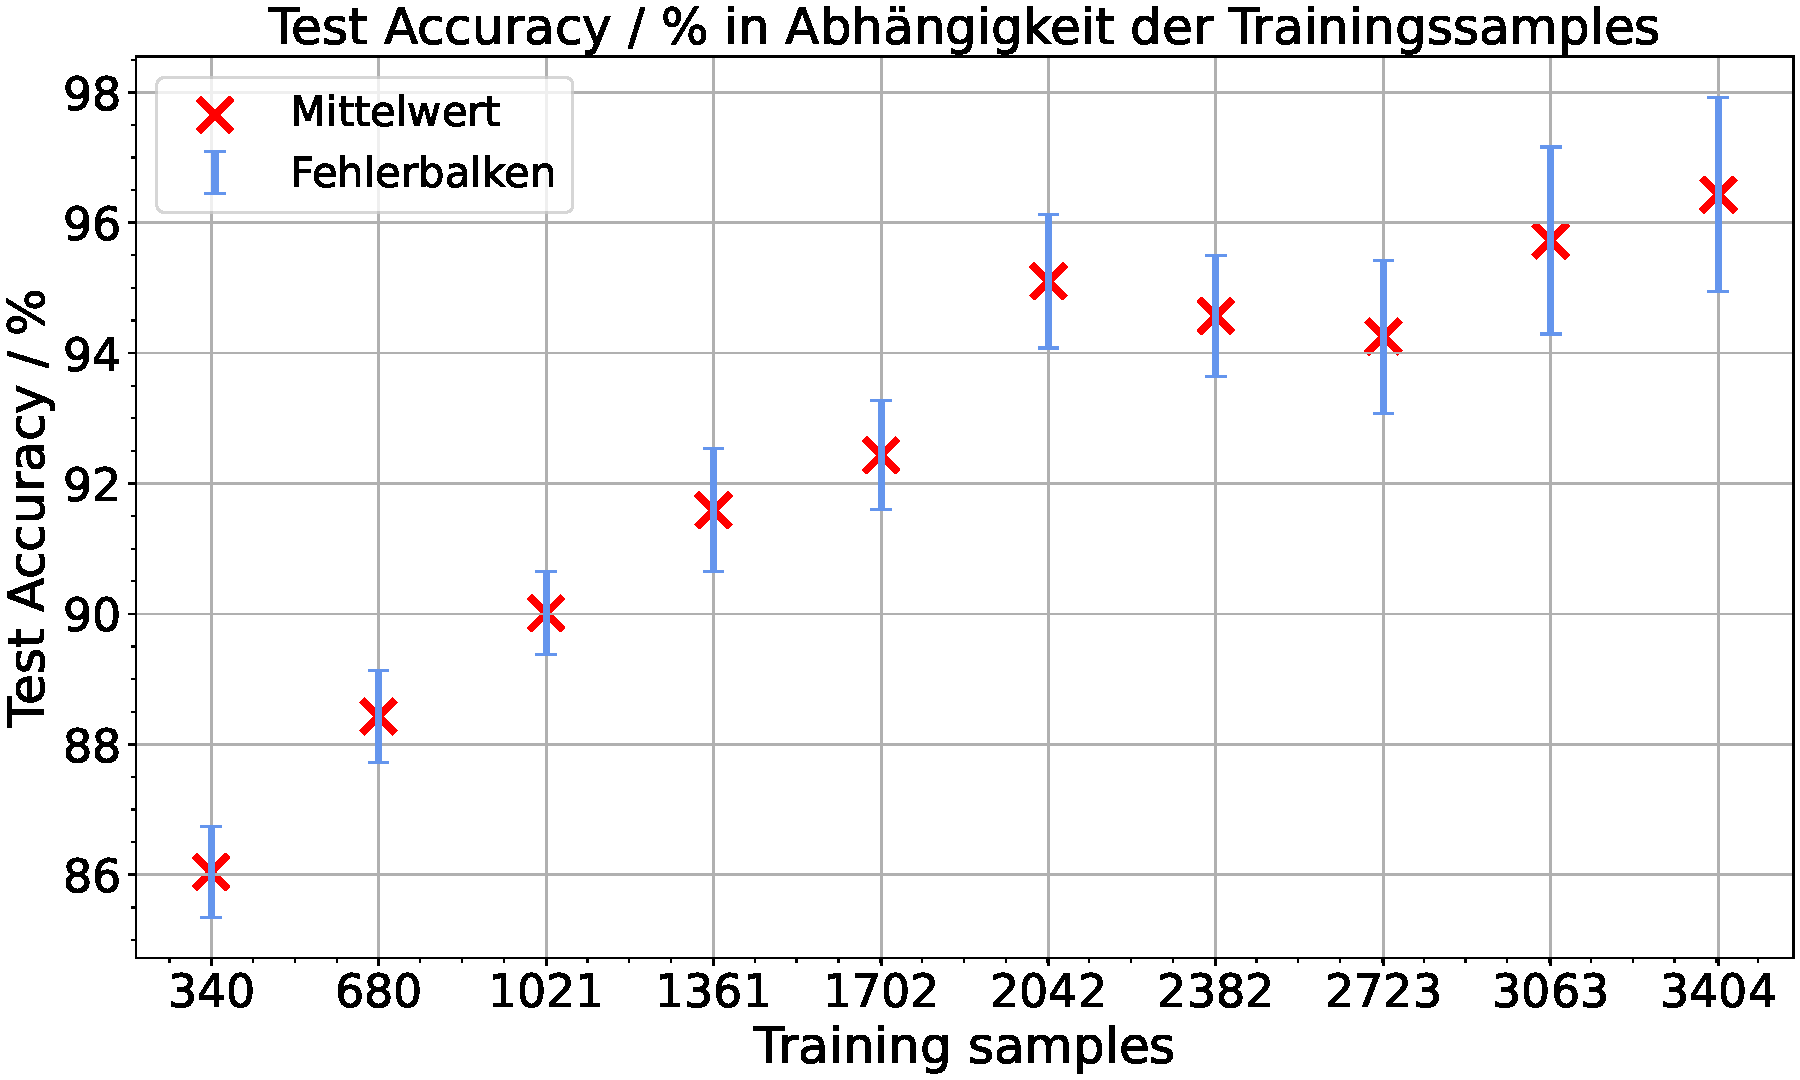
\includegraphics[width=\textwidth]{plots/Augm-Messungen-noTu-Tu_Accuracy_mean.pdf}
    \caption{Accuracy}
    \label{fig:augmentation_accuracy}
  \end{subfigure}
  \begin{subfigure}[b]{0.48\textwidth}
    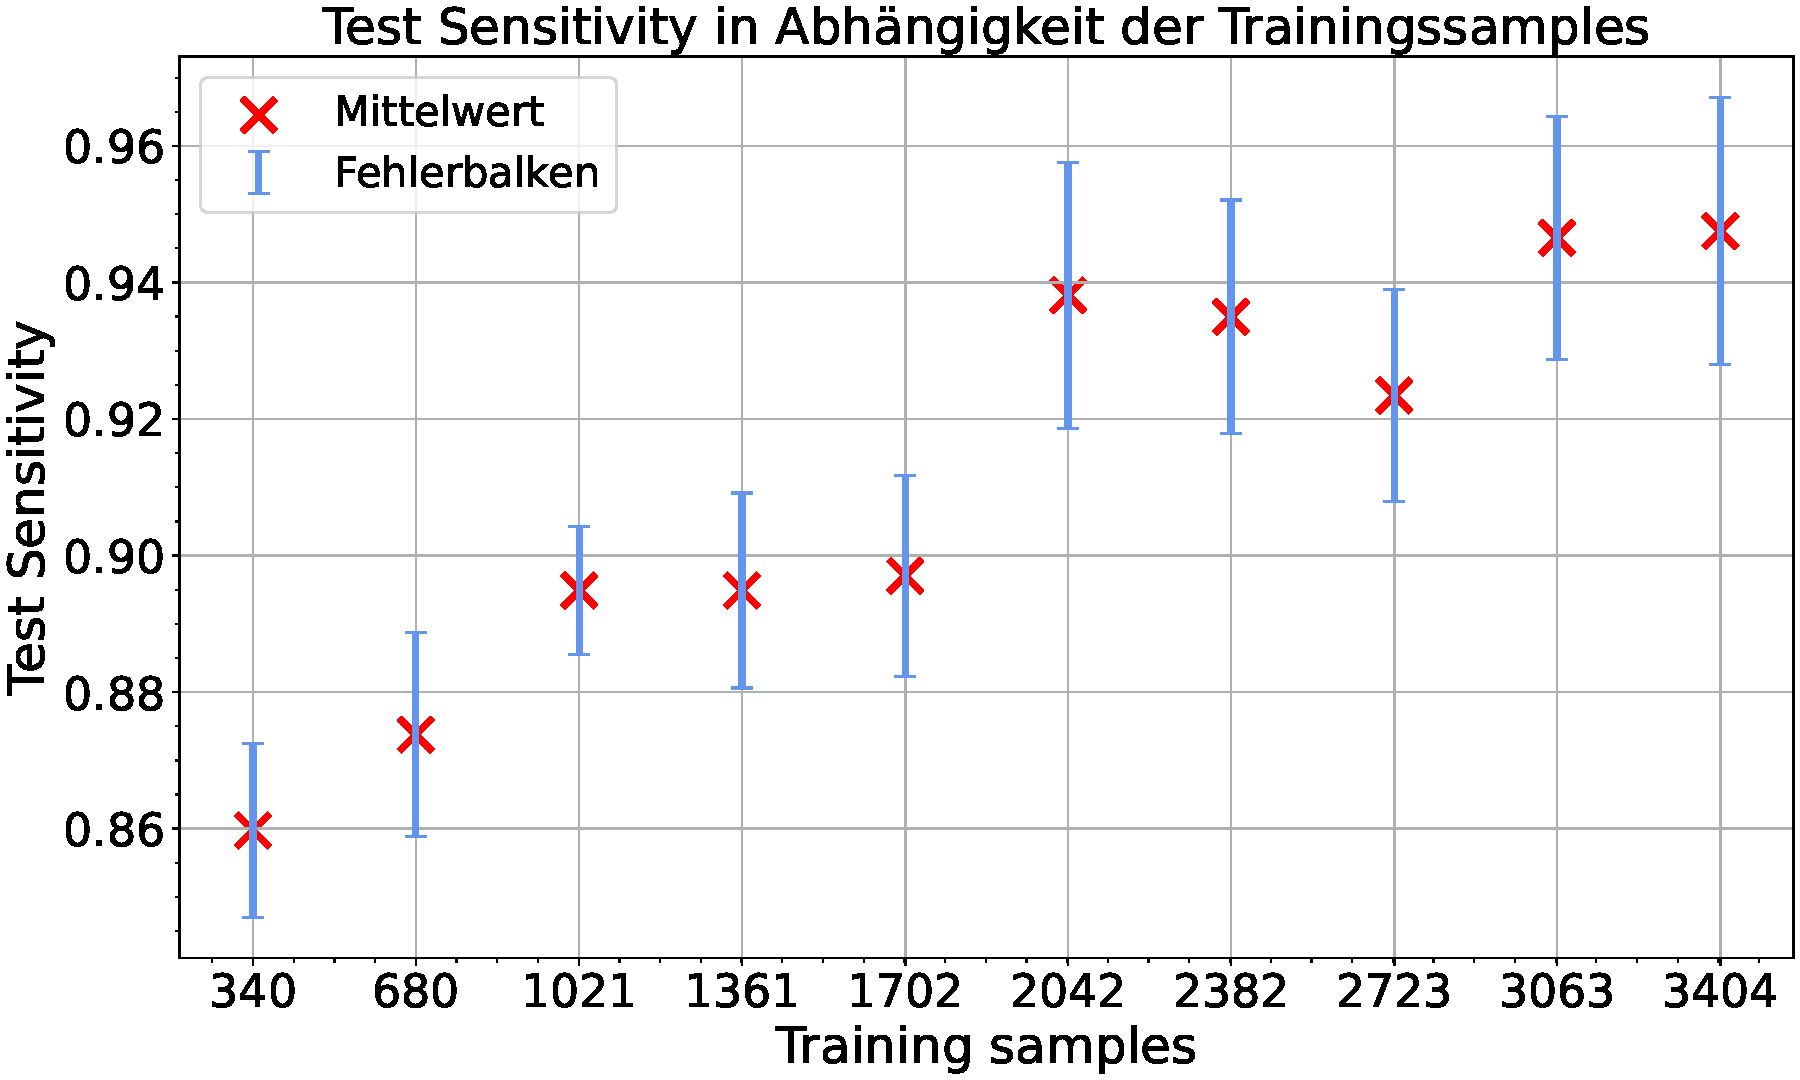
\includegraphics[width=\textwidth]{plots/Augm-Messungen-noTu-Tu_Sensitivity_mean.pdf}
    \caption{Sensitivity}
    \label{fig:augmentation_sensitivity}
  \end{subfigure}
  \begin{subfigure}[b]{0.48\textwidth}
    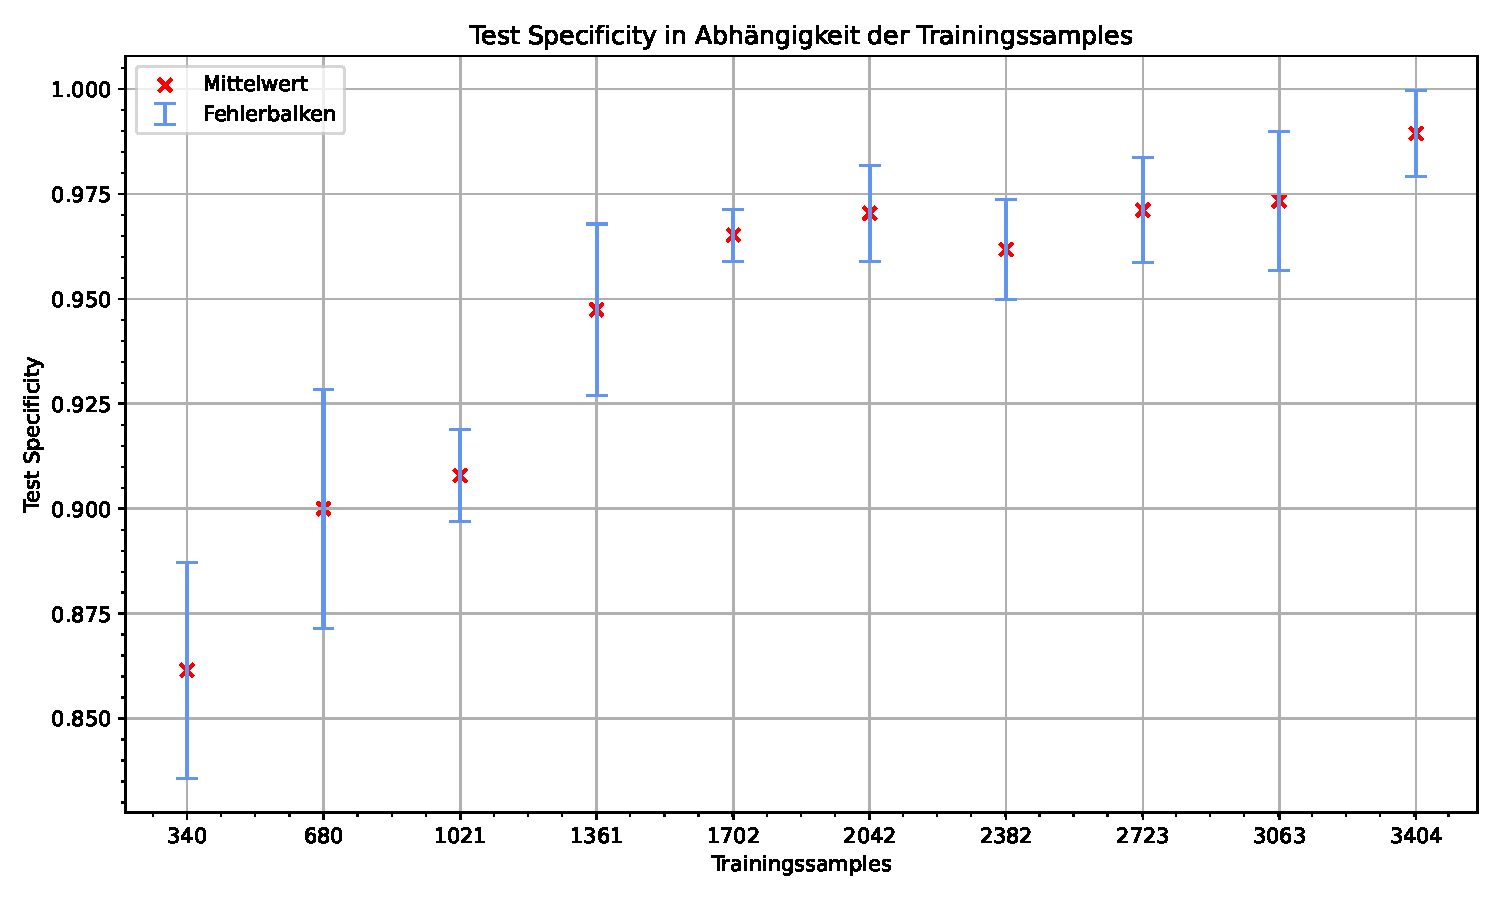
\includegraphics[width=\textwidth]{plots/Augm-Messungen-noTu-Tu_Specificity_mean.pdf}
    \caption{Specificity}
    \label{fig:augmentation_specificity}
  \end{subfigure}
  \caption{Verlauf der Metriken bei unterschiedlichen Anzahl an Training samples, unter Verwendung von Augmentation, für die Klassifikation zwischen no Tumor und Tumor.}
  \label{fig:augmentation_tu}
\end{figure}
\begin{table}[H]
    \centering
    {\small
        \begin{tabular}{cccc}
            \toprule
            Training sample & Accuracy/\% & Sensitivity & Specificity\\
            \midrule
            340  & $86.0435 \pm 0.6923$ & $0.8597 \pm 0.0127$ & $0.8615 \pm 0.0257$\\
            680  & $88.4273 \pm 0.7041$ & $0.8738 \pm 0.0150$ & $0.9000 \pm 0.0284$\\
            1021 & $90.0099 \pm 0.6376$ & $0.8949 \pm 0.0093$ & $0.9079 \pm 0.0110$\\
            1361 & $91.5925 \pm 0.9418$ & $0.8949 \pm 0.0143$ & $0.9474 \pm 0.0204$\\
            1702 & $92.4332 \pm 0.8357$ & $0.8970 \pm 0.0147$ & $0.9652 \pm 0.0062$\\
            2042 & $95.1039 \pm 1.0250$ & $0.9381 \pm 0.0195$ & $0.9704 \pm 0.0115$\\
            2382 & $94.5697 \pm 0.9296$ & $0.9350 \pm 0.0171$ & $0.9617 \pm 0.0119$\\
            2723 & $94.2532 \pm 1.1726$ & $0.9234 \pm 0.0155$ & $0.9711 \pm 0.0125$\\
            3063 & $95.7270 \pm 1.4340$ & $0.9465 \pm 0.0178$ & $0.9733 \pm 0.0166$\\
            3404 & $96.4293 \pm 1.4880$ & $0.9475 \pm 0.0195$ & $0.9894 \pm 0.0103$\\
            \bottomrule
        \end{tabular}}
  \caption{Mittelwert und Standardabweichung der Metriken bei Reduzierung der Training samples unter Verwendung von Augmentation.}
  \label{tab:augm-tunotu}
\end{table}

\subsection{Reduzierung der Tumor samples}
Für die Untersuchung der Netzwerkleistung bei Reduzierung einer Klasse, wurde die Anzahl an Tumor samples reduziert.
Der Verlauf der drei Metriken, sowie die Werte werden in der Abbildung \ref{fig:reduzierung_tumorsamples} und in der Tabelle \ref{tab:red_tu} dargestellt.
Die Accuracy steigt mit zunehmender Anzahl an samples bis zu maximal \SI{96.7458}{\percent} für 1702 Training samples.
Bei 1276 und 2128 samples sinkt sie auf ungefähr \SI{92}{\percent} ab. 
Die Sensitivity bleibt von 212 bis 851 Tumor samples konstant bei ca. \SI{0.9}{}.
Danach steigt sie leicht an und erreicht bei 1915 verwendeten Bildern einen Wert von \SI{0.9515}{}.
Auch hier sinkt bei der Verwendung aller Tumor Bilder die Sensitivity wieder ab.
Die Specificity steigt mit höherer sample Anzahl und konvergiert gegen \SI{1.0}.
Bei 212 und 1276 Tumor samples tritt eine hohe Standardabweichung für die Specificity und Accuracy auf.
Zusätzlich kommt es auch bei 2128, für die Accuracy und für die Sensitivity, zu einer große Abweichung
Bei den Klassengrößen 
In Runs bei denen 212 und 1276 Tumor samples verwendet wurden, lag die Specificity, 
sowie bei 2128 Tumor samples die Sensitivity bei 0.
\begin{figure}[H]
  \centering
  \begin{subfigure}[b]{0.48\textwidth}
    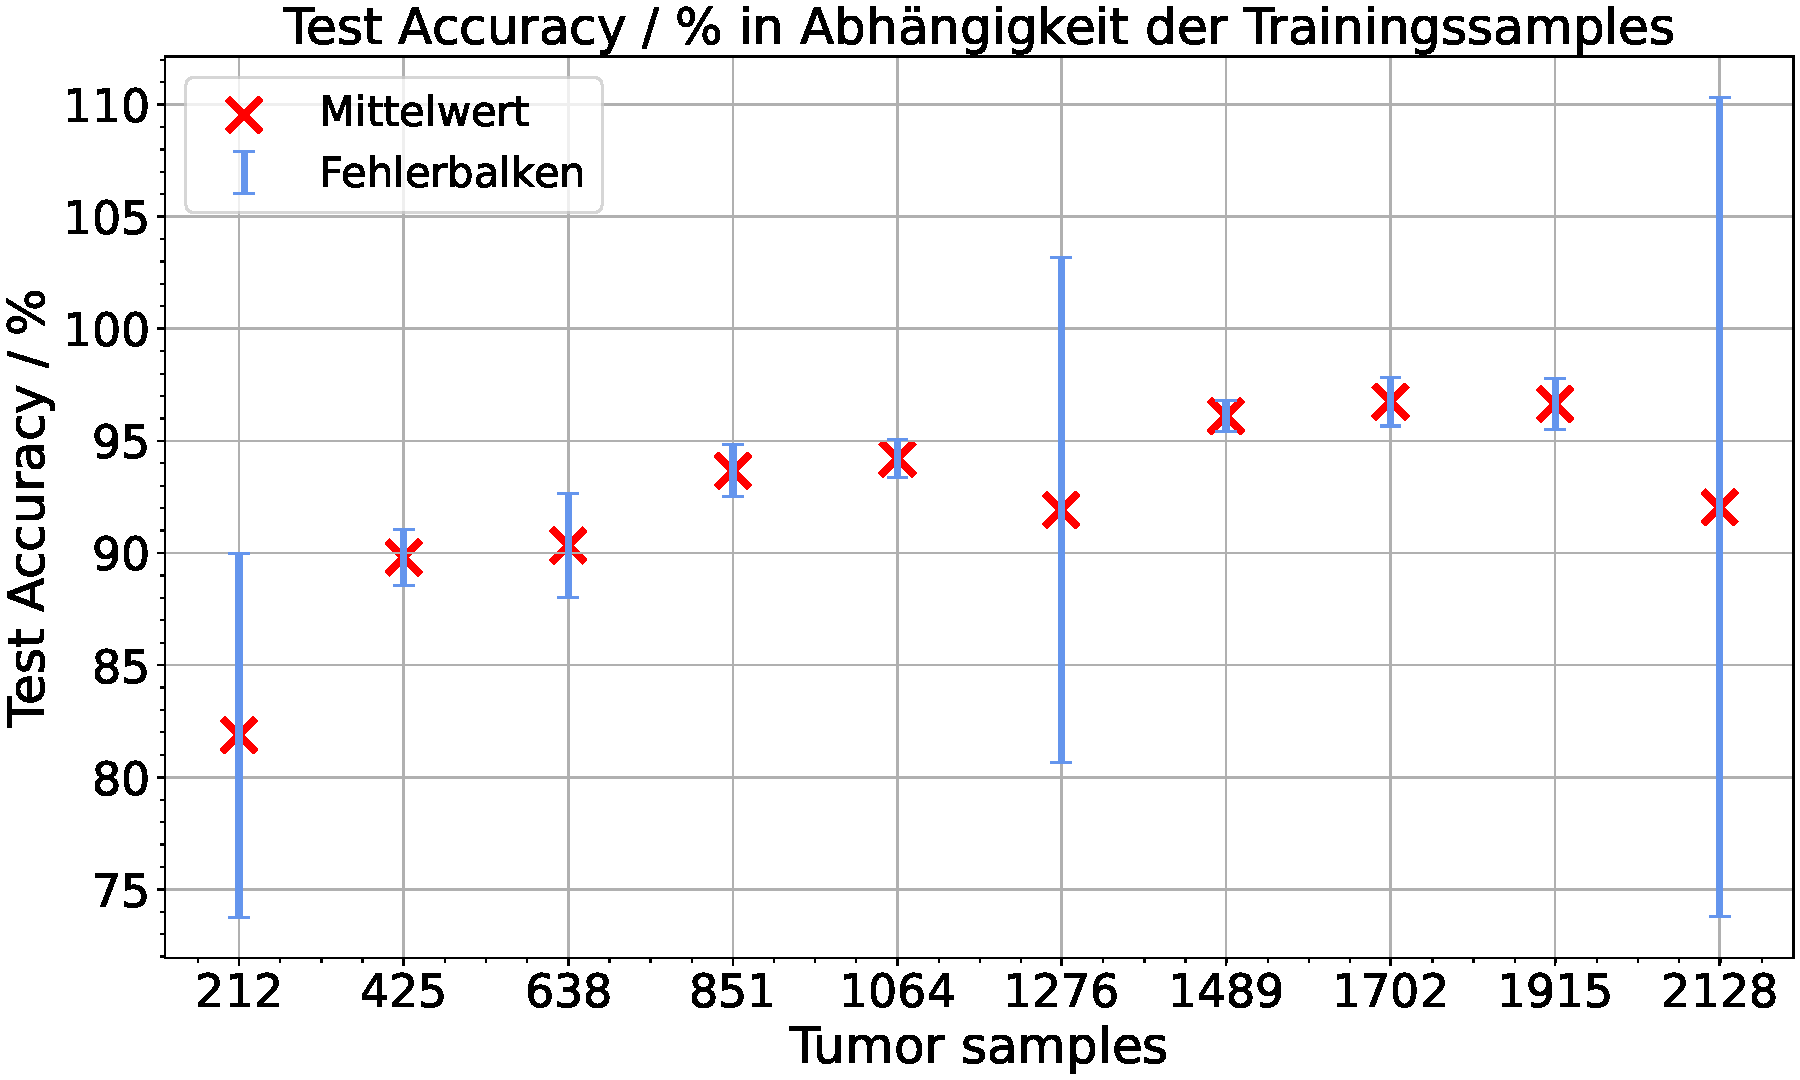
\includegraphics[width=\textwidth]{plots/neu Reduzierung-Tu + Balance_Accuracy_mean.pdf}
    \caption{Accuracy}
    \label{fig:reduzierung_tu_accuracy}
  \end{subfigure}
  \begin{subfigure}[b]{0.48\textwidth}
    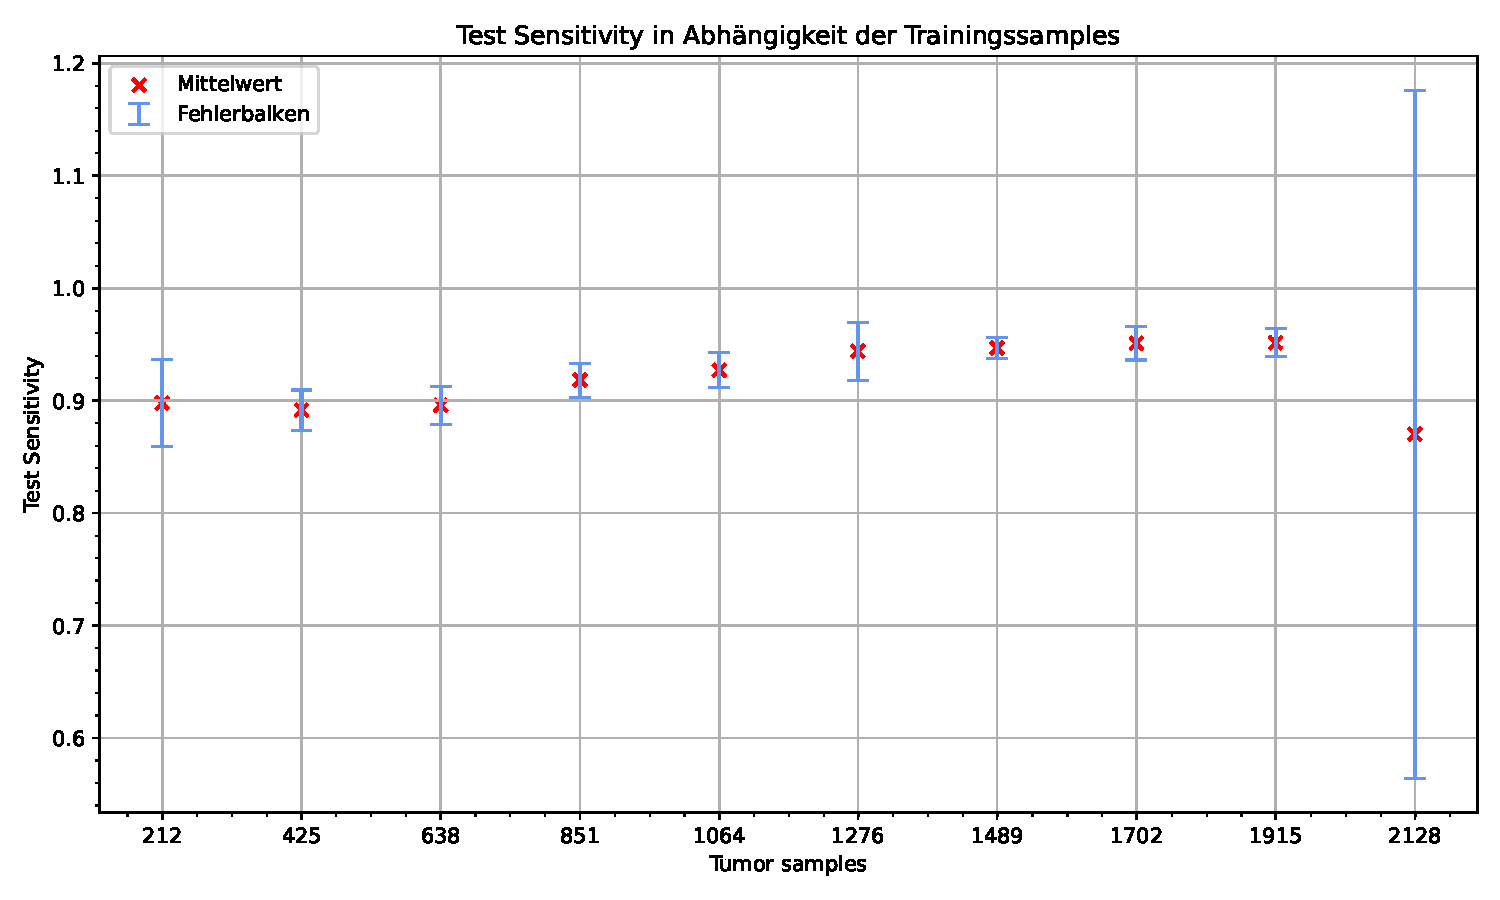
\includegraphics[width=\textwidth]{plots/neu Reduzierung-Tu + Balance_Sensitivity_mean.pdf}
    \caption{Sensitivity}
    \label{fig:reduzierung_tu_sensitivity}
  \end{subfigure}
  \begin{subfigure}[b]{0.48\textwidth}
    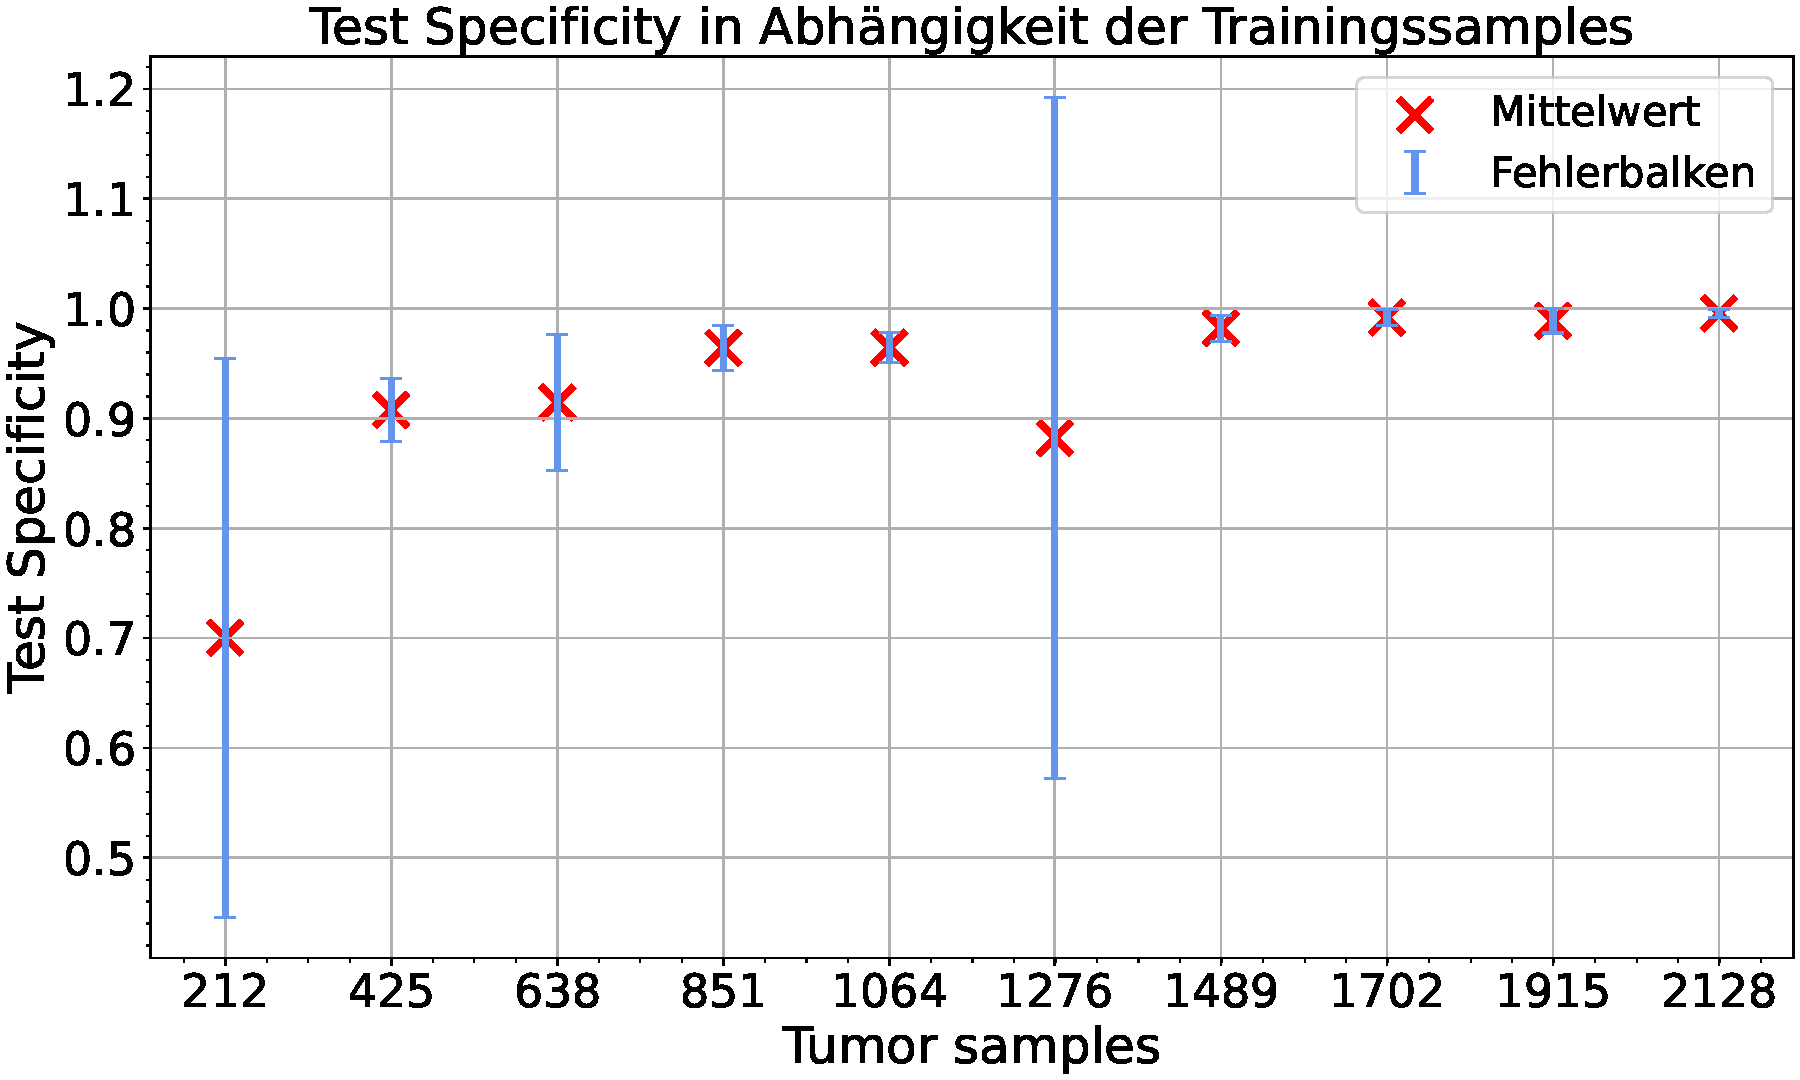
\includegraphics[width=\textwidth]{plots/neu Reduzierung-Tu + Balance_Specificity_mean.pdf}
    \caption{Specificity}
    \label{fig:reduzierung_tu_specificity}
  \end{subfigure}
  \caption{Metriken bei Reduktion der Tumor samples.}
  \label{fig:reduzierung_tumorsamples}
\end{figure}
\begin{table}[H]
    \centering
     {\small
        \begin{tabular}{cccc}
            \toprule
            Training sample & Accuracy/\% & Sensitivity & Specificity\\
            \midrule
            212  & $81.8694 \pm 8.1081$ & $0.8979 \pm 0.0389$ & $0.7002 \pm 0.2544$\\
            425  & $89.8022 \pm 1.2611$ & $0.8916 \pm 0.0179$ & $0.9077 \pm 0.0285$\\
            638  & $90.3363 \pm 2.3230$ & $0.8959 \pm 0.0170$ & $0.9146 \pm 0.0622$\\
            851  & $93.6696 \pm 1.1535$ & $0.9183 \pm 0.0151$ & $0.9642 \pm 0.0203$\\
            1064 & $94.2038 \pm 0.8486$ & $0.9271 \pm 0.0156$ & $0.9644 \pm 0.0135$\\
            1276 & $91.9189 \pm 11.273$ & $0.9441 \pm 0.0258$ & $0.8820 \pm 0.3100$\\
            1489 & $96.1029 \pm 0.6919$ & $0.9469 \pm 0.0095$ & $0.9822 \pm 0.0118$\\
            1702 & $96.7458 \pm 1.0820$ & $0.9512 \pm 0.0150$ & $0.9919 \pm 0.0069$\\
            1915 & $96.6469 \pm 1.1234$ & $0.9515 \pm 0.0124$ & $0.9889 \pm 0.0111$\\
            2128 & $92.0376 \pm 18.269$ & $0.8701 \pm 0.3058$ & $0.9956 \pm 0.0036$\\
            \bottomrule
        \end{tabular}}
  \caption{Mittelwert und Standardabweichung der Metriken bei der Reduzierung der Tumor Klasse.}
  \label{tab:red_tu}
\end{table}
%%%%%%%%%%%%%%%%%%%%%%%%%%%%%%%%%%%%%%%%%%%%%%%%%%%%%%%%%%%%%%%%%%%%%%
\section{Klassifizierung zwischen Glioma und Meningioma}
\subsection{Hyperparameter}
Für die Ermittlung der Hyperparameter werden die fünf Runs mit den niedrigsten Validation loss betrachtet.
Der Verlauf wird in der Abbildung \ref{fig:val_loss gli-men} dargestellt.
Die dazugehörigen Parameter und die Accuracy, Sensitivity und Specificity des Validierung Datensatzes werden in der Tabelle \ref{tab:hyperp-gli men} aufgelistet.
\begin{figure}[H]
  \centering
  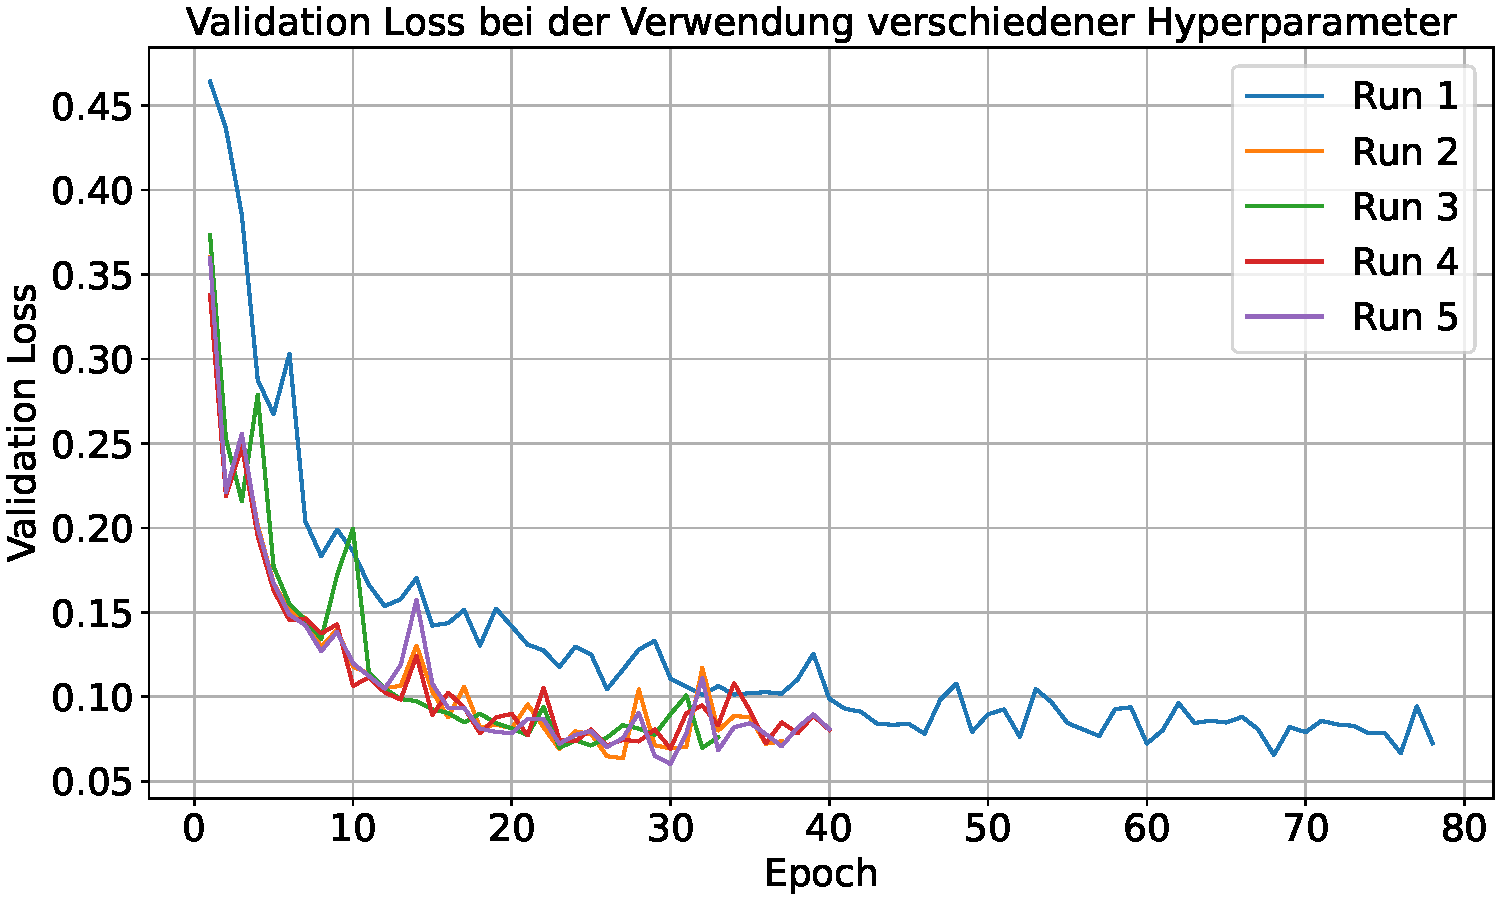
\includegraphics[scale=0.4]{plots/Val_loss_Gli_Men.pdf}
  \caption{Darstellung des validation loss bei der Verwendung verschiedener Hyperparameter.}
  \label{fig:val_loss gli-men}
\end{figure}
\begin{table}[H]
    \centering
    \resizebox{\textwidth}{!}{%
        \begin{tabular}{cccccccc}
            \toprule
            Runs & Batch Größe & Lernrate & Dropout & Validation Loss & Accuracy/$\%$ & Sensitivity & Specificity \\
            \midrule
            1 & 128 & 0.01  & 0.55 & 0.18943 & 92.29323 & 0.95402 & 0.89299 \\
            2 & 64  & 0.005 & 0.3  & 0.22499 & 93.23308 & 0.96935 & 0.89668 \\
            3 & 16  & 0.0005& 0.55 & 0.23146 & 93.98496 & 0.92720 & 0.95203 \\
            4 & 16  & 0.005 & 0.5  & 0.23453 & 92.66917 & 0.95402 & 0.90037 \\
            5 & 16  & 0.0005& 0.5  & 0.23829 & 93.42105 & 0.94253 & 0.92620 \\
            \bottomrule
        \end{tabular}
    }
  \caption{Die fünf Runs mit dem niedrigsten validation loss sowie deren verwendete Hyperparameter und aufgezeichnete Metriken.}
  \label{tab:hyperp-gli men}
\end{table}
Der erste Run besitzt zwar den niedrigsten validation loss, jedoch auch die niedrigste Accuracy und Specificity.
Der höchste Wert der Accuracy und Specificity tritt bei Run 3 auf
Aufgrund dessen werden in den folgenden Trainingsdurchläufen die Hyperparameter von Run 3 verwendet.
\subsection{Reduzierung der Trainingsdaten}
In Abbildung \ref{fig:gli-men-reduktion} ist der Verlauf der Accuracy, Sensitivity und Specificity bei der Reduktion der Training samples dargestellt.
Die dazu gehörigen Werte werden in der Tabelle \ref{tab:Red-gli-men} dargestellt.
Die drei Metriken steigen, mit zunehmender Anzahl an samples. 
Bei 851 Training samples sinken die Werte etwas, bevor sie anschließend wieder ansteigen.
Die Accuracy erhöht sich von \SI{76.4191}{\percent}, bei 231 Training samples auf \SI{92.3102}{\percent} bei 2128 Training samples.
Die Sensitivity steigt bis 1702 Training samples auf \SI{0.9186}{} an und bleibt anschließend weitgehend konstant zwischen \SI{0.9114}{} und \SI{0.9255}{}.
Die Specificity nimmt bis 1064 Training samples zu und bleibt bis 1277 konstant. 
Danach sinkt diese kurzzeitig etwas und steigt anschließend wieder an. 
Ab 1915 Training samples bleibt die Specificity stabil bei ungefähr \SI{0.92}{}.
\begin{figure}[H]
  \centering
  \begin{subfigure}[b]{0.48\textwidth}
    \centering
    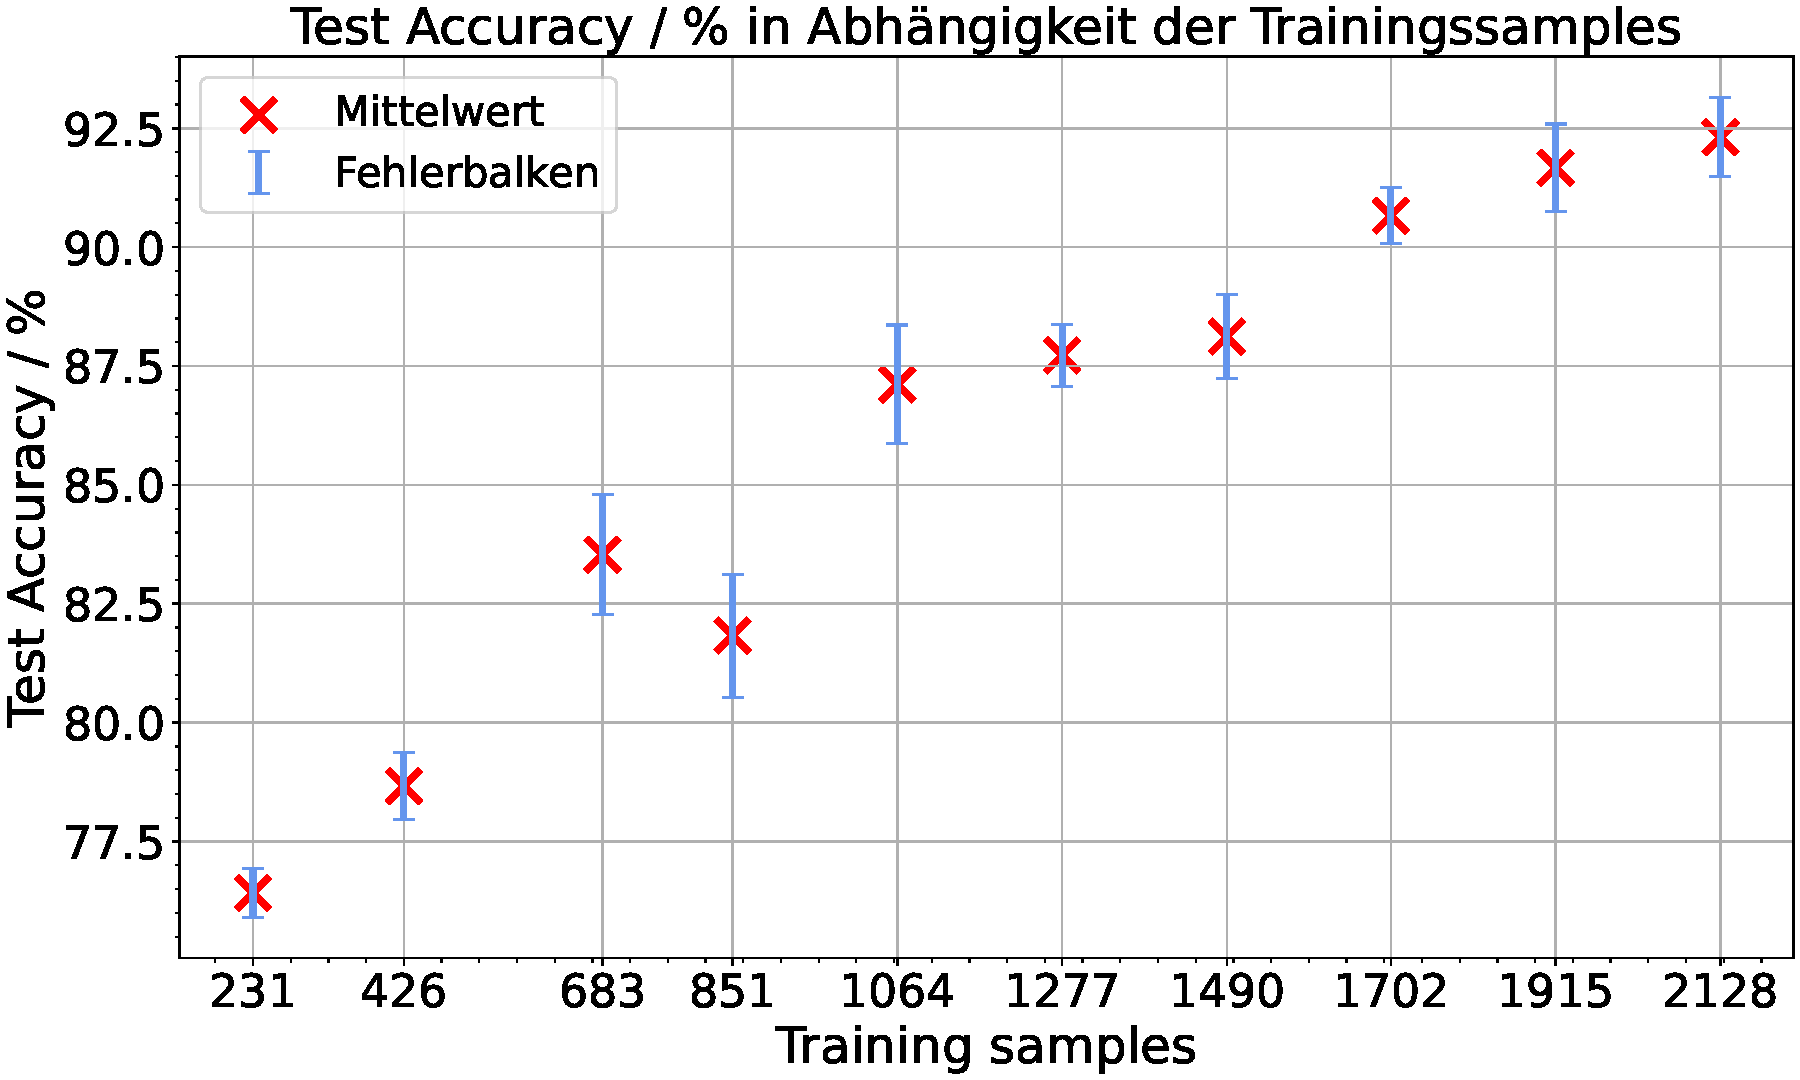
\includegraphics[width=\textwidth]{plots/3-Messungen-Gli-Men_Accuracy_mean.pdf}
    \caption{Accuracy}
    \label{fig:gli-men-acc}
  \end{subfigure}
  \begin{subfigure}[b]{0.48\textwidth}
    \centering
    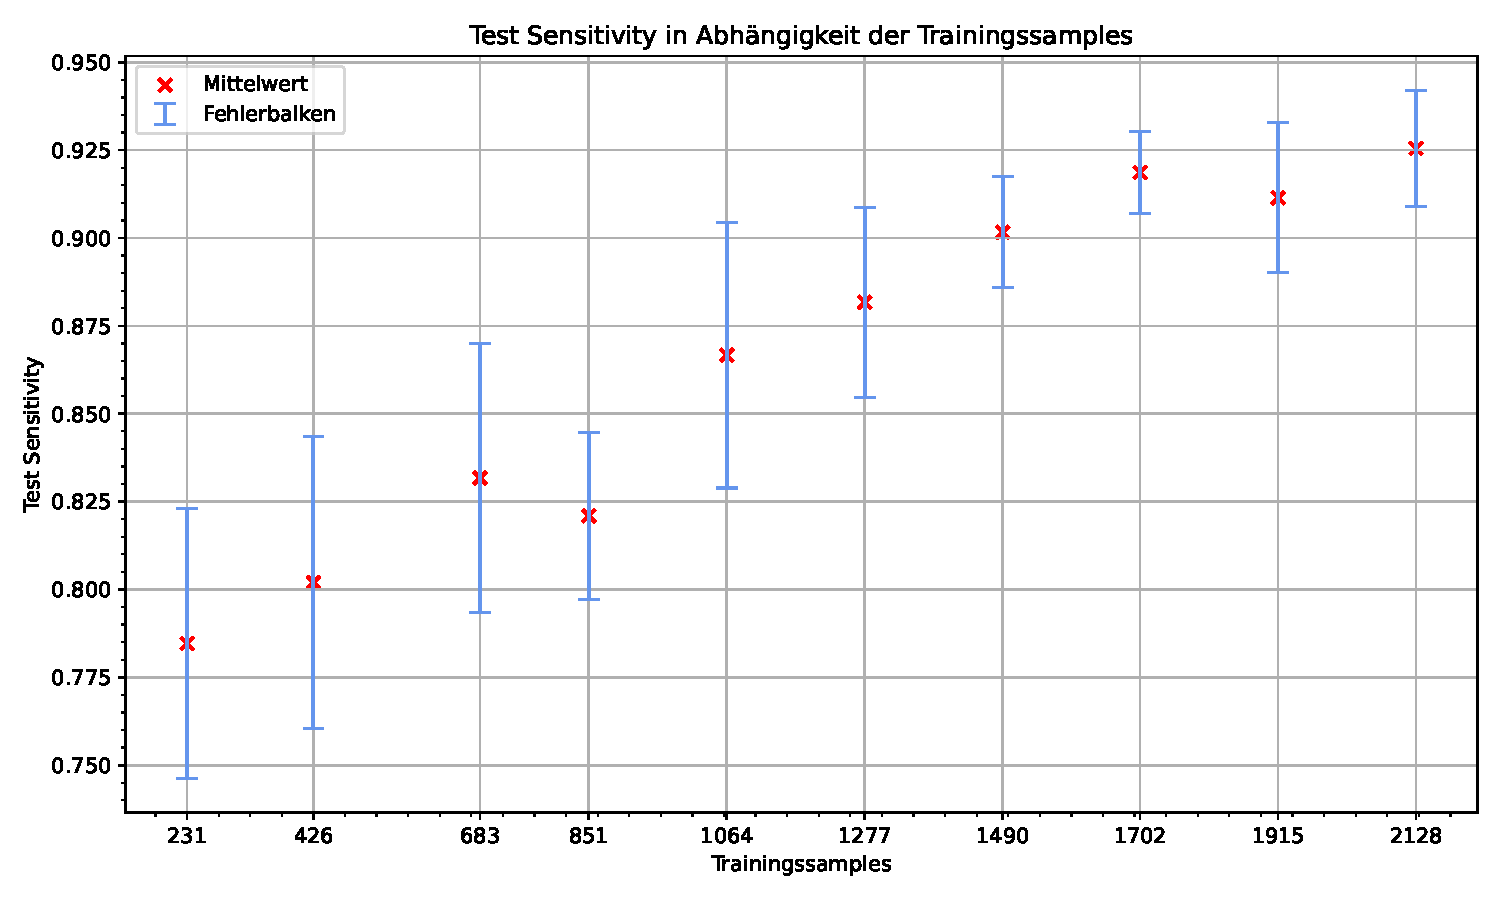
\includegraphics[width=\textwidth]{plots/3-Messungen-Gli-Men_Sensitivity_mean.pdf}
    \caption{Sensitivität}
    \label{fig:gli-men-sens}
  \end{subfigure}
  \begin{subfigure}[b]{0.48\textwidth}
    \centering
    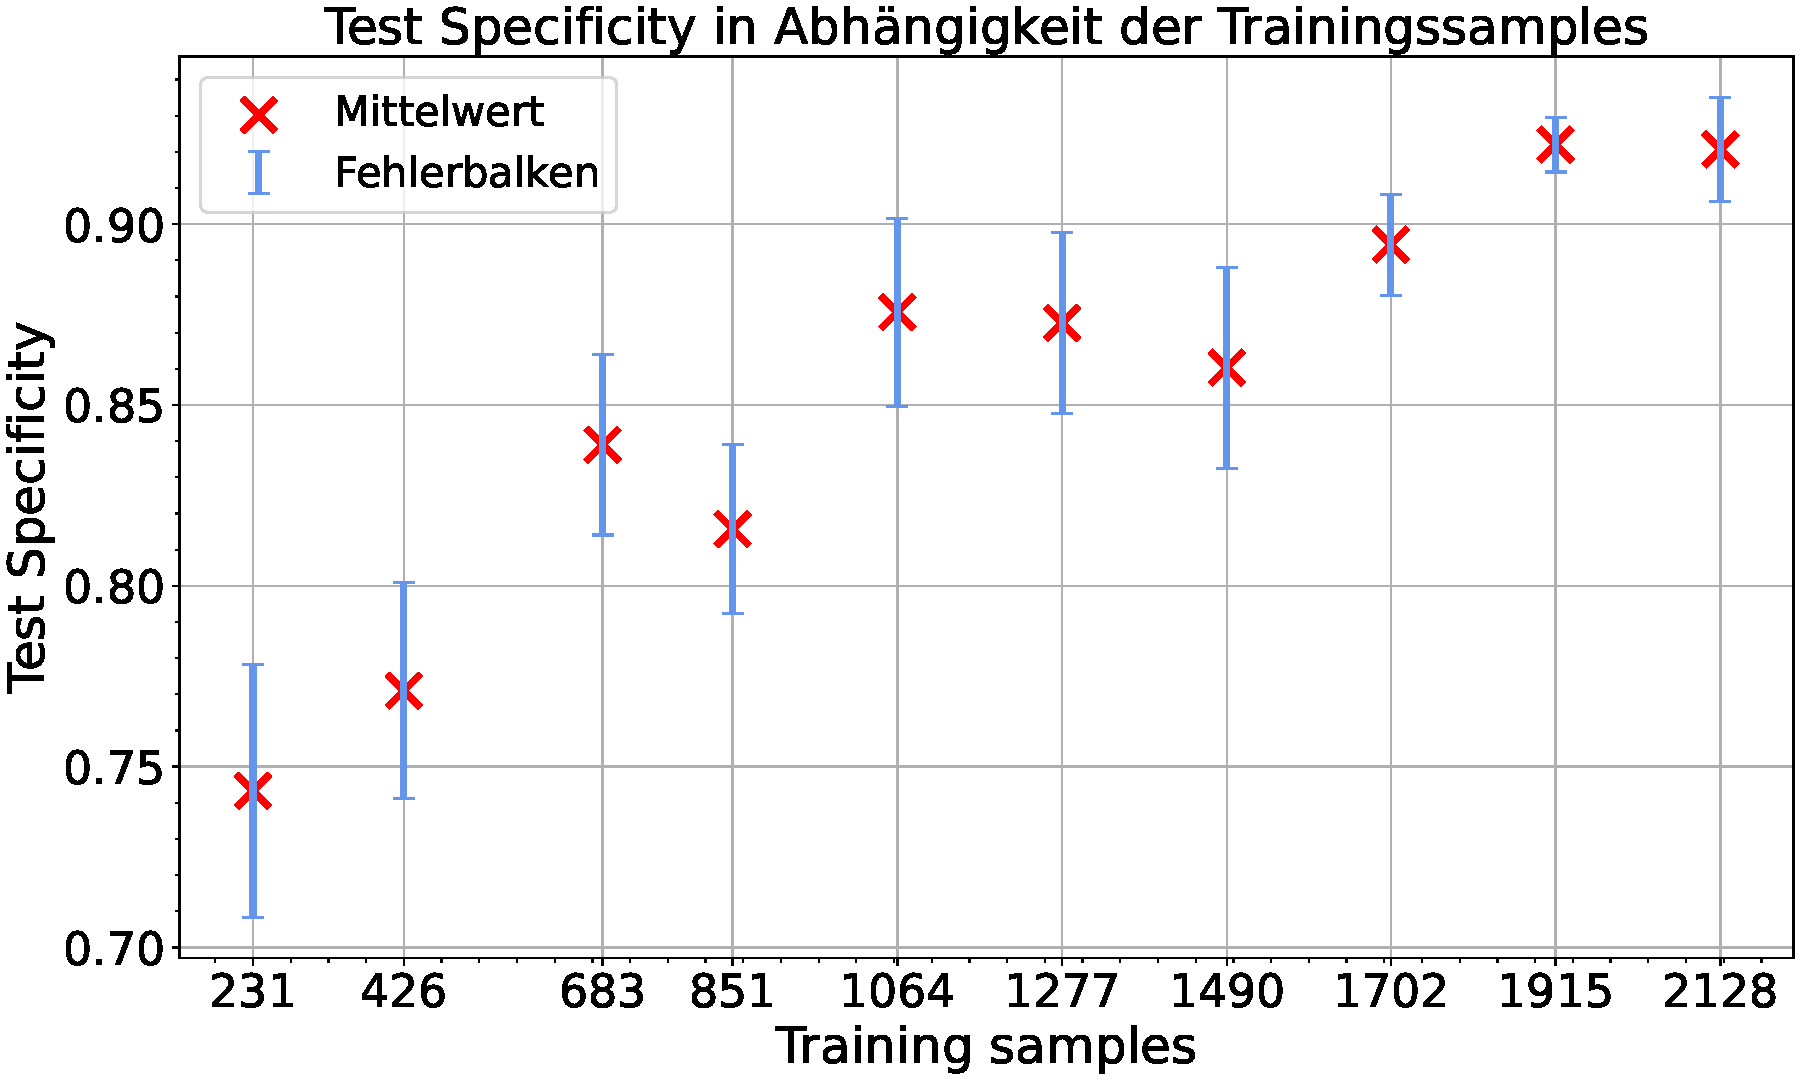
\includegraphics[width=\textwidth]{plots/3-Messungen-Gli-Men_Specificity_mean.pdf}
    \caption{Specificity}
    \label{fig:gli-men-spec}
  \end{subfigure}
  \caption{Verlauf der Metriken bei der Reduzierung der Training samples für die Klassifikation zwischen Glioma und Meningioma.}
  \label{fig:gli-men-reduktion}
\end{figure}
\begin{table}[H]
    \centering
    {\small
        \begin{tabular}{cccc}
            \toprule
            Training sample & Accuracy/$\%$ & Sensitivity & Specificity\\
            \midrule
            231  & $76.4191 \pm 0.5068$ & $0.7846 \pm 0.0383$ & $0.7433 \pm 0.0349$\\
            426  & $78.6634 \pm 0.7046$ & $0.8020 \pm 0.0414$ & $0.7710 \pm 0.0298$\\
            683  & $83.5314 \pm 1.2658$ & $0.8317 \pm 0.0383$ & $0.8390 \pm 0.0249$\\
            851  & $81.8317 \pm 1.2934$ & $0.8209 \pm 0.0238$ & $0.8157 \pm 0.0233$\\
            1064 & $87.1122 \pm 1.2506$ & $0.8667 \pm 0.0378$ & $0.8757 \pm 0.0260$\\
            1277 & $87.7228 \pm 0.6518$ & $0.8817 \pm 0.0270$ & $0.8727 \pm 0.0250$\\
            1490 & $88.1188 \pm 0.8903$ & $0.9016 \pm 0.0158$ & $0.8603 \pm 0.0278$\\
            1702 & $90.6601 \pm 0.5934$ & $0.9186 \pm 0.0117$ & $0.8943 \pm 0.0140$\\
            1915 & $91.6667 \pm 0.9212$ & $0.9114 \pm 0.0214$ & $0.9220 \pm 0.0076$\\
            2128 & $92.3102 \pm 0.8313$ & $0.9255 \pm 0.0165$ & $0.9207 \pm 0.0143$\\            
            \bottomrule
        \end{tabular}}
  \caption{Mittelwert und Standardabweichung für die Reduzierung der Training samples.}
  \label{tab:Red-gli-men}
\end{table}
\vspace{-3.5em}
\subsection{Augmentation}
%\vspace{-0.5em}
Unter Verwendung von Augmentation wurden die Training samples reduziert.
Der Verlauf der Metriken ist in der Abbildung \ref{fig:gli-men-augm} dargestellt,
die entsprechenden Werte sind in der Tabelle \ref{tab:gli-men-augm} zu finden.
Die Accuracy steigt kontinuierlich mit der verwendeten Sample Anzahl.
Zu beginn liegt sie bei \SI{75.8746}{\percent} für 212 samples. 
Bei der Nutzung aller verfügbaren Trainingsdaten erreicht \SI{92.1947}{\percent}.
Die Sensitivity steigt zunächst bis zu 425 Bildern an, sinkt anschließend etwas bei 638 Samples, nimmt danach jedoch wieder zu.
Ab 1702 samples bleibt sie konstant bei \SI{0.9101}{}, bevor sie bei 2128 Training samples auf \SI{0.9261} ansteigt. 
Der Anstieg der Specificity erfolgt konstant bis 1064 Training sample und flacht anschließend ab.
Bei 2128 Samples wird eine Specificity von \SI{0.9177}{} erreicht.
\begin{table}[H]
    \centering
    {\small
        \begin{tabular}{cccc}
            \toprule
            Training sample & Accuracy/$\%$ & Sensitivity & Specificity\\
            \midrule
            212  & $75.8746 \pm 0.6115$ & $0.7801 \pm 0.0564$ & $0.7370 \pm 0.0656$ \\
            425  & $79.7195 \pm 0.4362$ & $0.8199 \pm 0.0147$ & $0.7740 \pm 0.0162$ \\
            638  & $80.6931 \pm 0.5663$ & $0.7958 \pm 0.0170$ & $0.8183 \pm 0.0085$ \\
            851  & $81.5512 \pm 0.9834$ & $0.8170 \pm 0.0228$ & $0.8140 \pm 0.0134$ \\
            1064 & $86.4521 \pm 0.8212$ & $0.8526 \pm 0.0239$ & $0.8767 \pm 0.0191$ \\
            1276 & $87.9868 \pm 0.8479$ & $0.8768 \pm 0.0180$ & $0.8830 \pm 0.0202$ \\
            1489 & $89.0099 \pm 1.1930$ & $0.8886 \pm 0.0221$ & $0.8917 \pm 0.0196$ \\
            1702 & $90.7096 \pm 0.5612$ & $0.9101 \pm 0.0209$ & $0.9040 \pm 0.0175$ \\
            1915 & $91.2706 \pm 1.2037$ & $0.9101 \pm 0.0182$ & $0.9153 \pm 0.0121$ \\
            2128 & $92.1947 \pm 0.8837$ & $0.9261 \pm 0.0139$ & $0.9177 \pm 0.0123$ \\         
            \bottomrule
        \end{tabular}}
  \caption{Mittelwert und Standardabweichung der drei Metriken bei Reduzierung der Training samples unter Verwendung von Augmentation für die Klassifikation zwischen Glioma und Meningioma.}
  \label{tab:gli-men-augm}
\end{table}
\begin{figure}[H]
  \centering
  \begin{subfigure}[b]{0.48\textwidth}
    \centering
    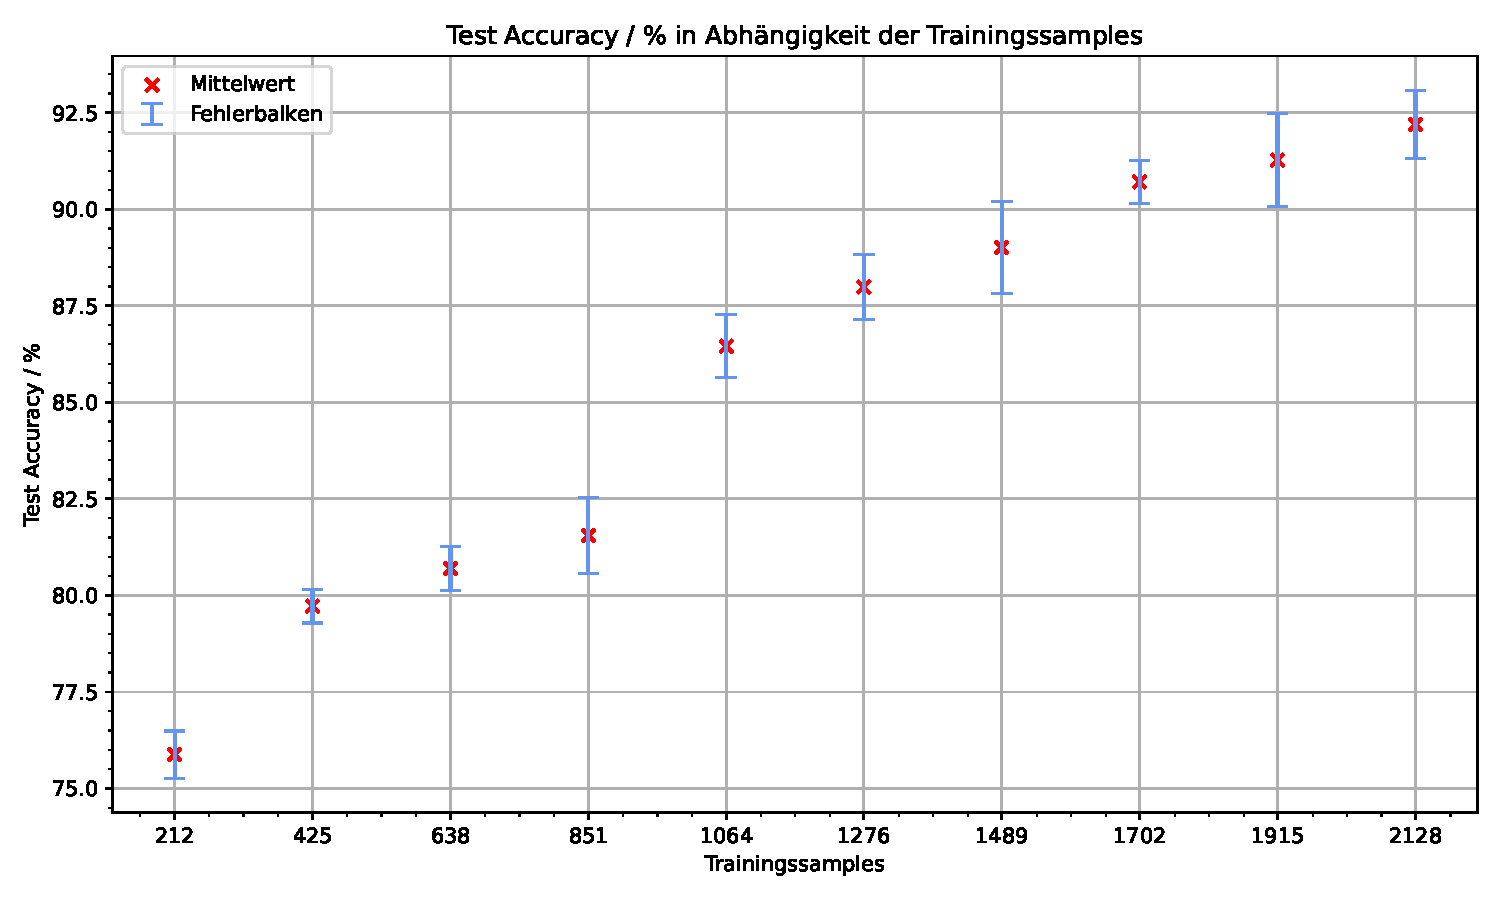
\includegraphics[width=\textwidth]{plots/Augm-Gli-Men_Accuracy_mean.pdf}
    \caption{Accuracy}
    \label{fig:augm-acc}
  \end{subfigure}
  \begin{subfigure}[b]{0.48\textwidth}
    \centering
    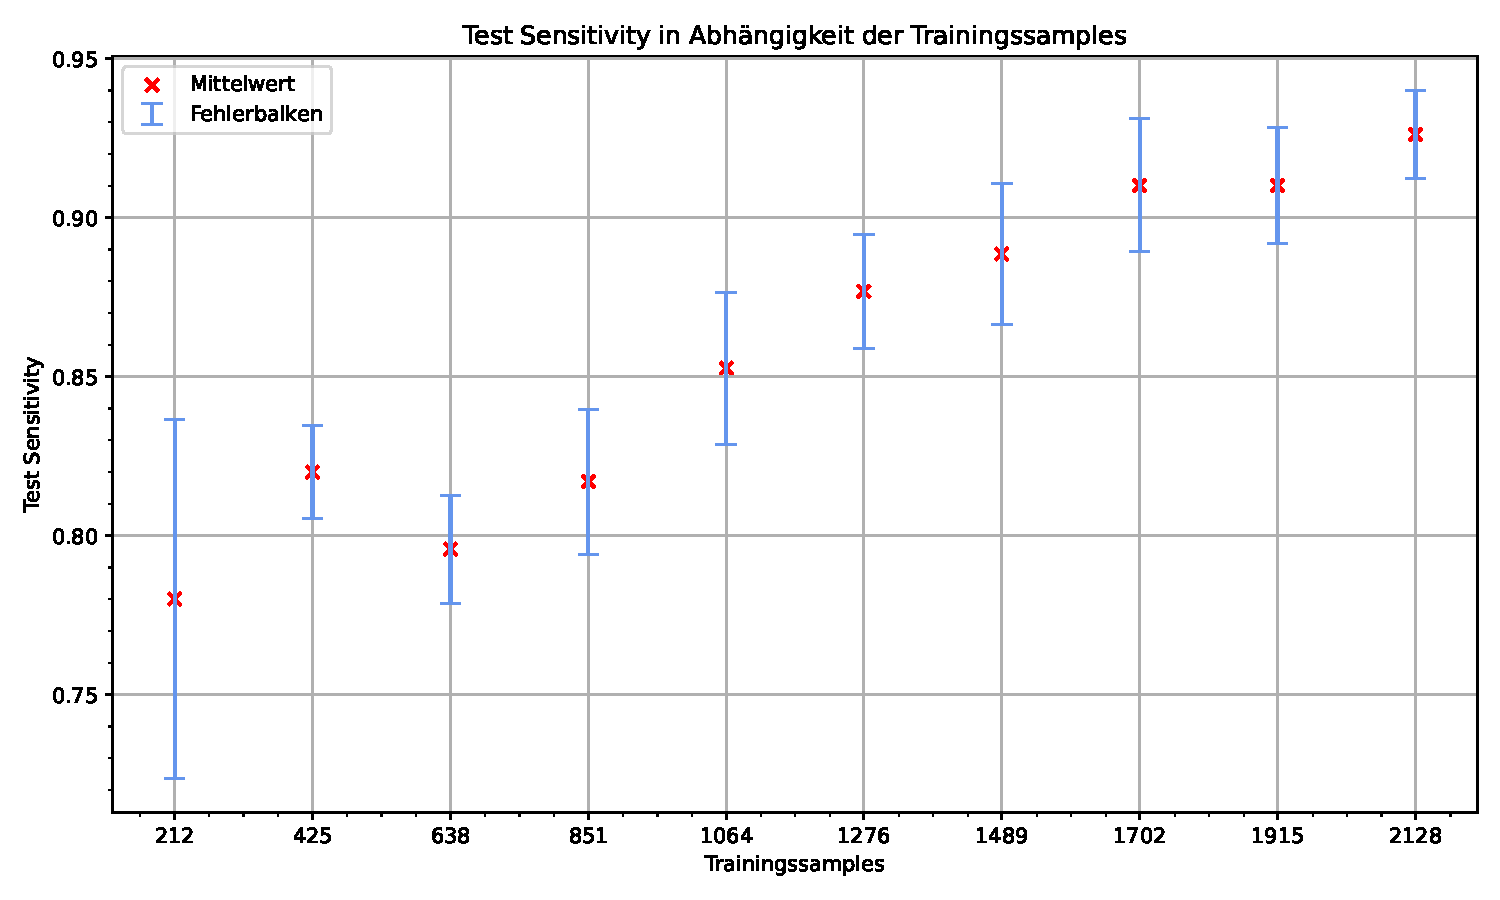
\includegraphics[width=\textwidth]{plots/Augm-Gli-Men_Sensitivity_mean.pdf}
    \caption{Sensitivität}
    \label{fig:augm-sens}
  \end{subfigure}
  \begin{subfigure}[b]{0.48\textwidth}
    \centering
    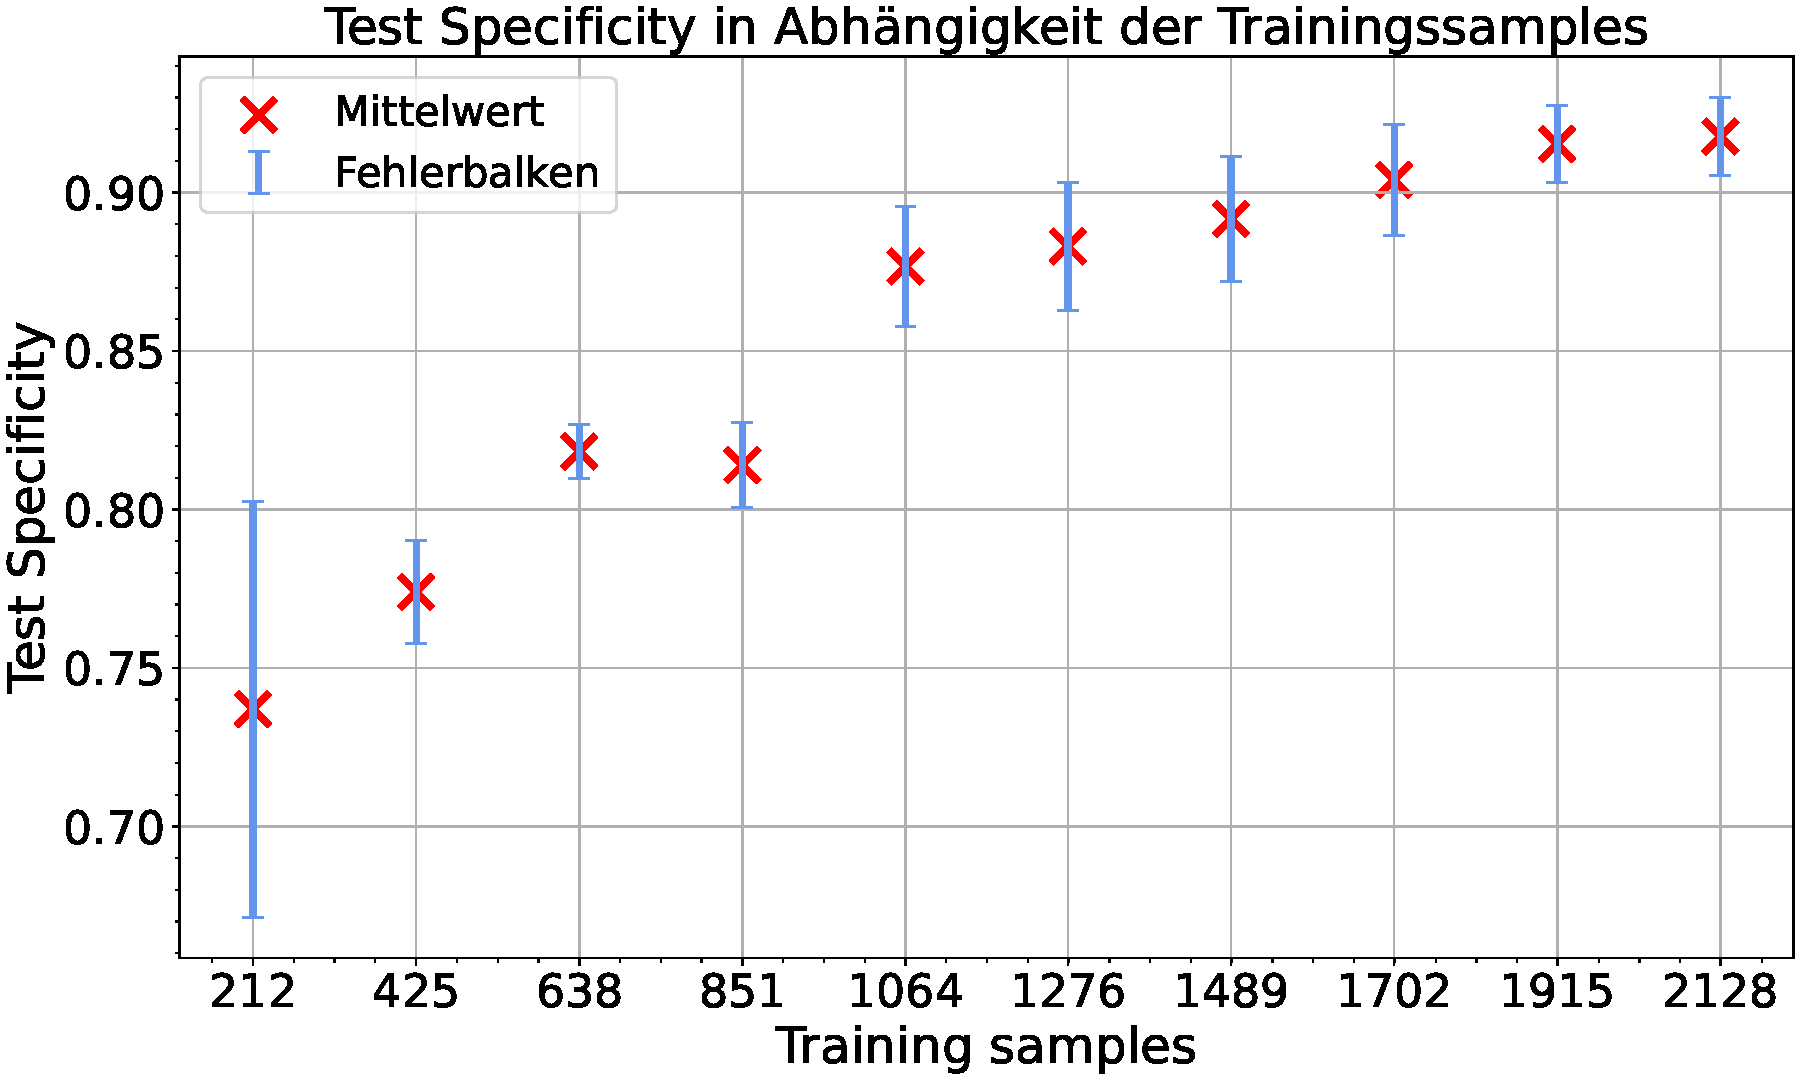
\includegraphics[width=\textwidth]{plots/Augm-Gli-Men_Specificity_mean.pdf}
    \caption{Specificity}
    \label{fig:augm-spec}
  \end{subfigure}
  \caption{Verlauf der Metriken bei Reduzierung der Training samples unter Verwendung von Augmentation für die Klassifikation zwischen Glioma und Meningioma.}
  \label{fig:gli-men-augm}
\end{figure}
\subsection{Reduzierung der Glioma sample}
Das Netzwerk wurde mit einer variierenden Anzahl an Glioma und konstanten Anzahl an Meningioma samples trainiert.
Der Verlauf der Metriken ist in der Abbildung \ref{fig:gli-men-gliored} dargestellt.
In der Tabelle \ref{tab:red-gli} sind die dargestellten Mittelwerte und Standardabweichungen aufgeführt. 
Es ist zu erkennen, dass die Accuracy und die Specificity zunächst bis zu 317 Glioma sample ansteigen und anschließend etwas absteigen.
Danach nehmen beide Werte erneut zu.
Die Accuracy wird ab 739 Glioma samples nahezu konstant bei etwa \SI{91}{\percent} und steigt bei 1057 Sample auf \SI{93.7459}{\percent} an.
Die Specificity schwankt im Bereich zwischen 739 und 951 Glioma samples zwischen \SI{0.8967}{} \SI{0.9177}{}.
Bei Verwendung aller verfügbaren Glioma samples erreicht sie einen Wert von \SI{0.9307}{}.
Die Sensitivity beträgt bei nur 105 verwendeten Glioma samples einen Wert von \SI{0.8056}{}.
Anschließende steigt sie deutlich an und schwankt im Bereich zwischen 211 und 951 Glioma samples zwischen \SI{0.8912}{} und \SI{0.9193}{}. 
Zum Schluss steigt sie bei 1057 Beispielen weiter auf \SI{0.9441}{}.
\begin{figure}[H]
  \centering
  \begin{subfigure}[b]{0.48\textwidth}
    \centering
    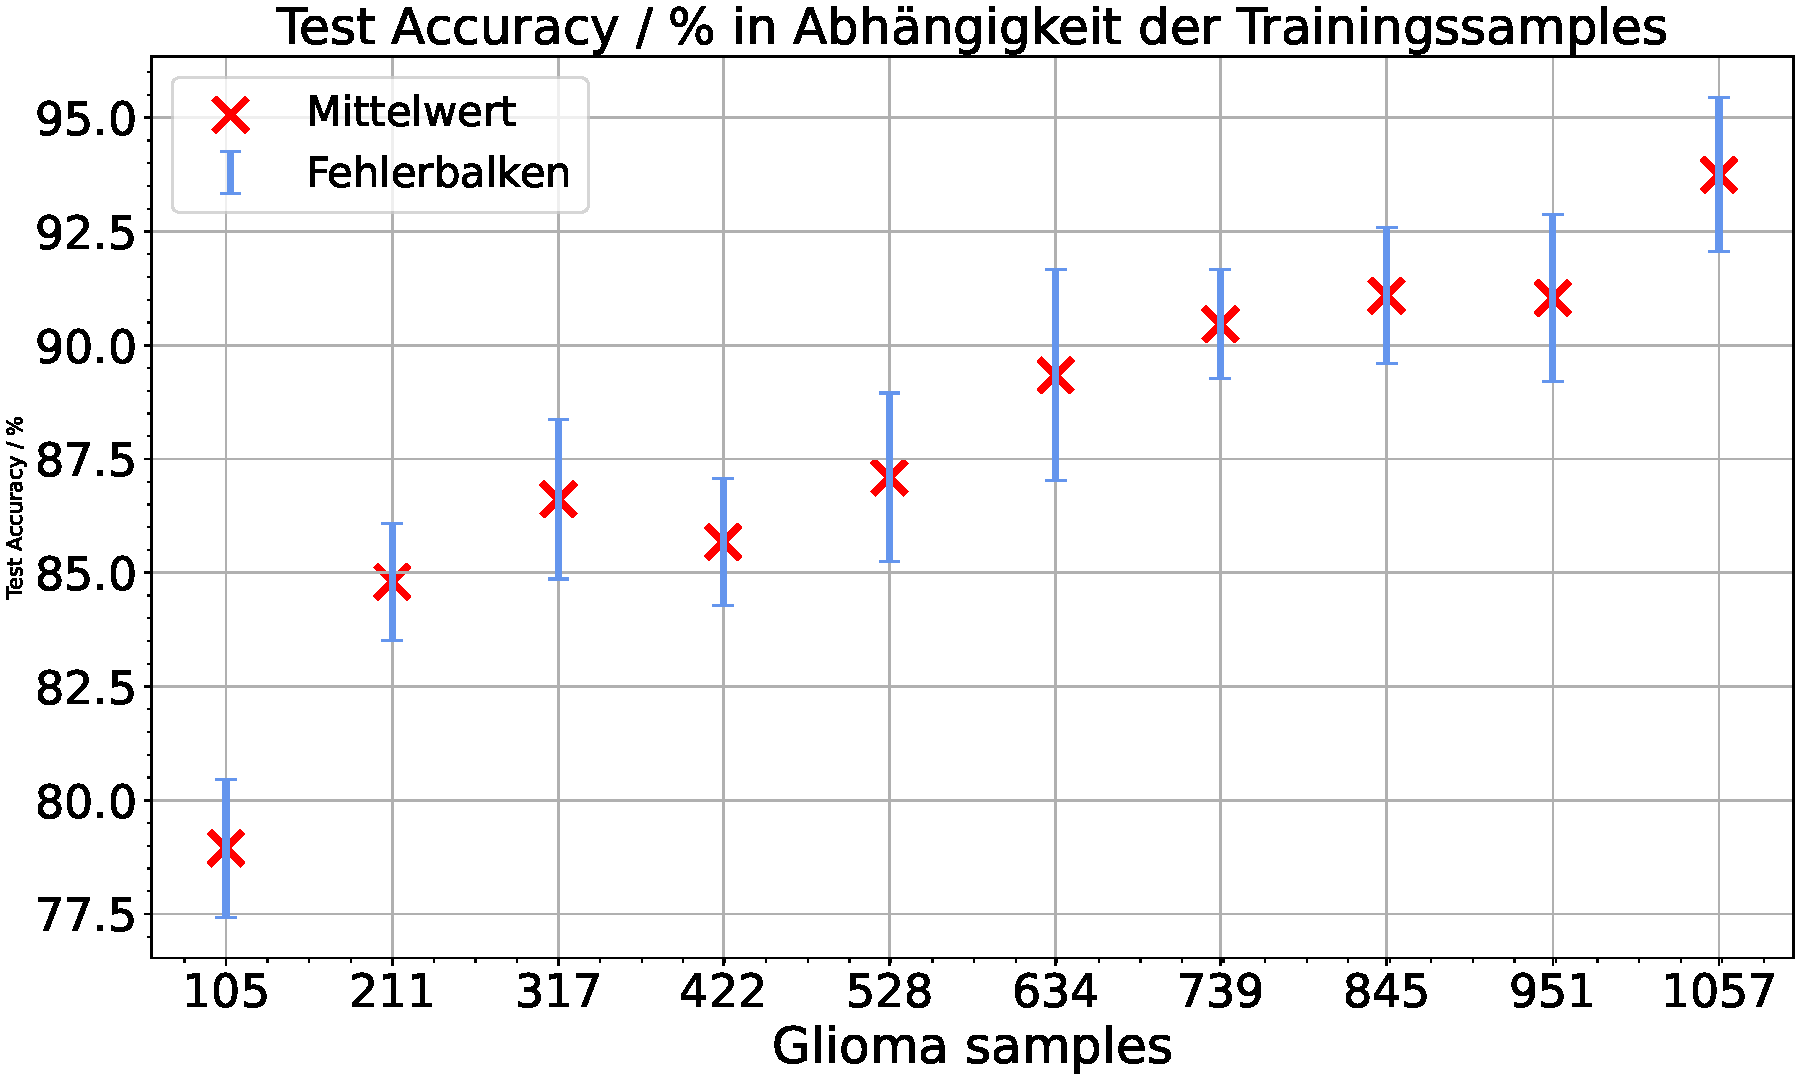
\includegraphics[width=\textwidth]{plots/Reduzierung-Gli + Balnce_Accuracy_mean.pdf}
    \caption{Accuracy}
    \label{fig:gli-red-acc}
  \end{subfigure}
  \begin{subfigure}[b]{0.48\textwidth}
    \centering
    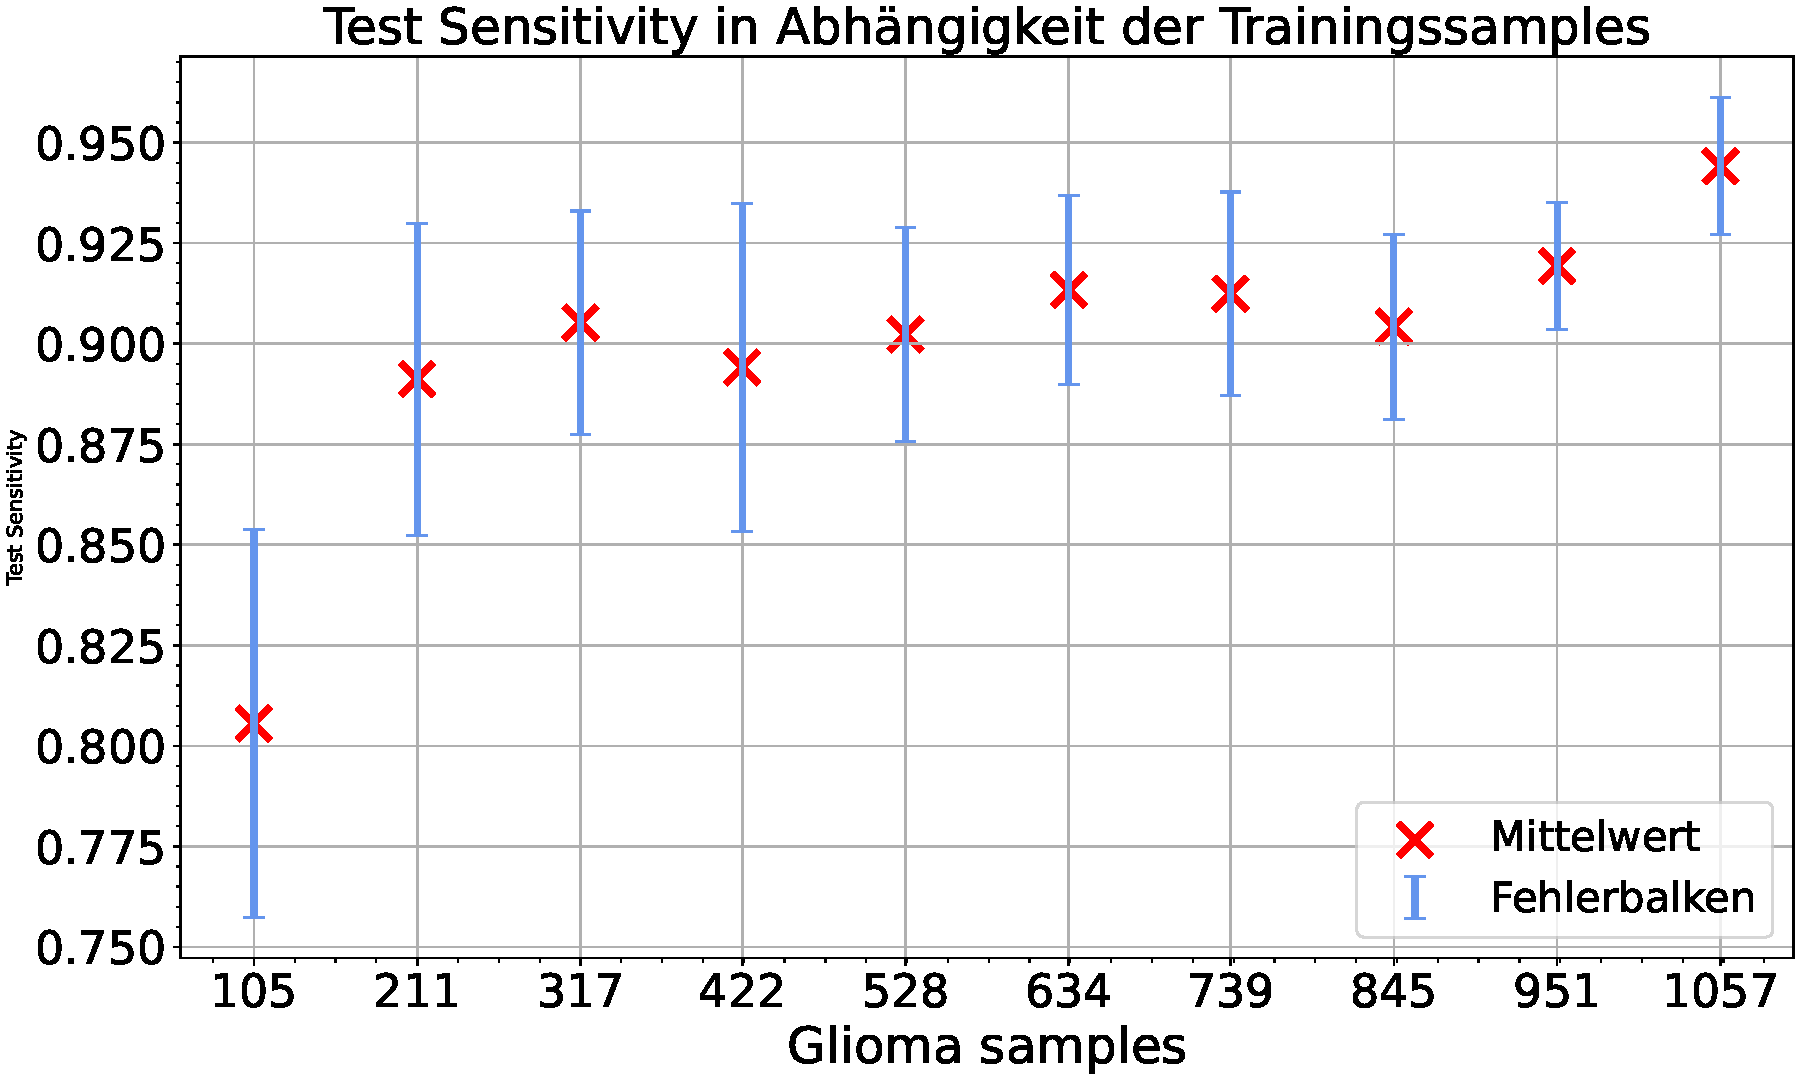
\includegraphics[width=\textwidth]{plots/Reduzierung-Gli + Balnce_Sensitivity_mean.pdf}
    \caption{Sensitivität}
    \label{fig:gli-red-sens}
  \end{subfigure}
  \begin{subfigure}[b]{0.48\textwidth}
    \centering
    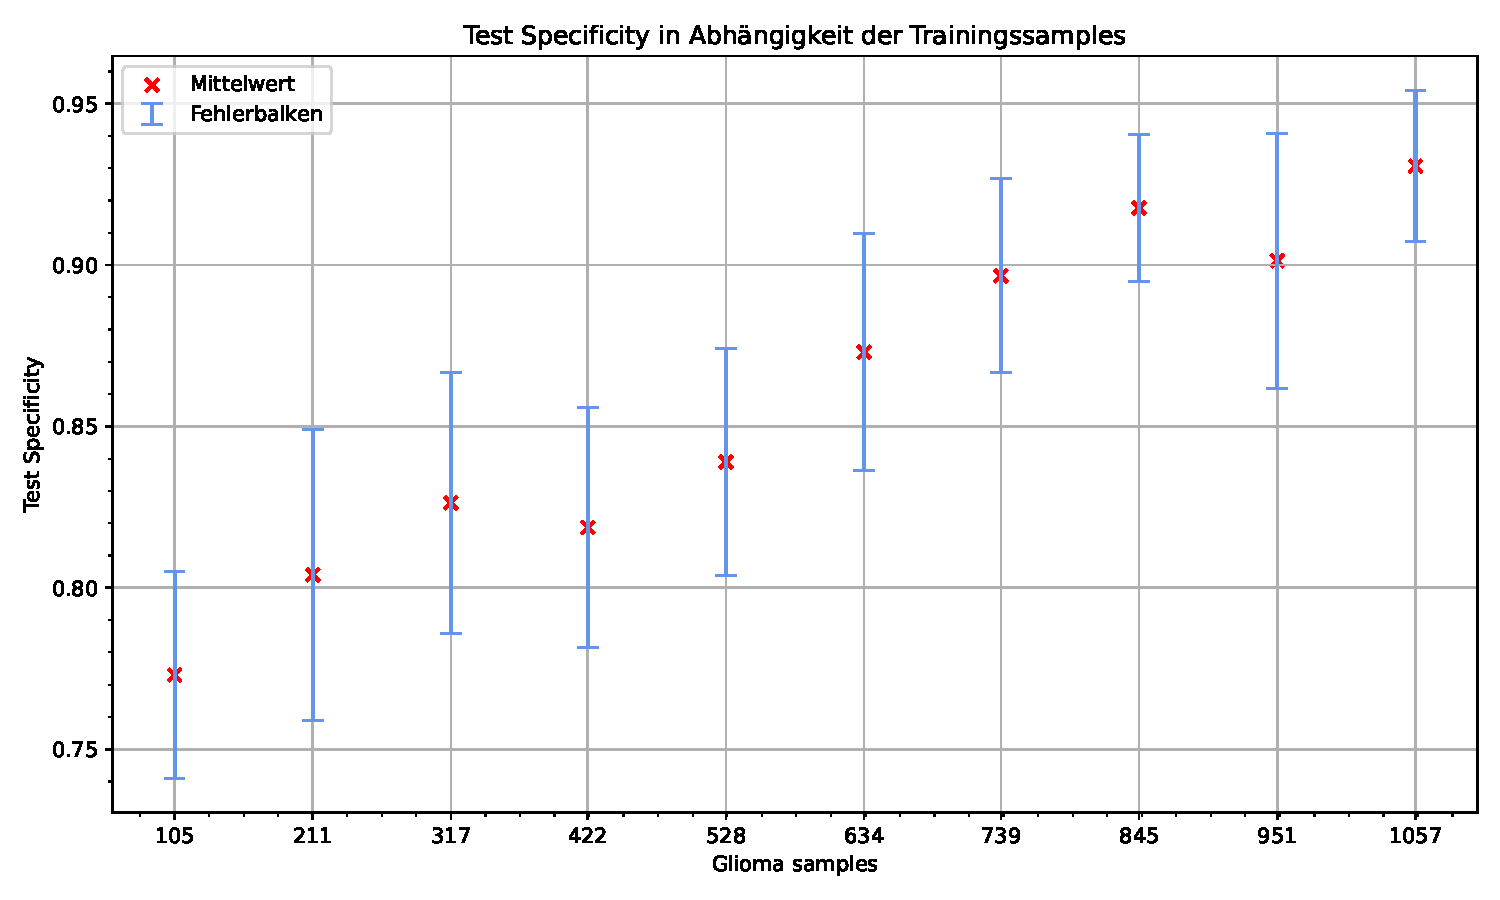
\includegraphics[width=\textwidth]{plots/Reduzierung-Gli + Balnce_Specificity_mean.pdf}
    \caption{Specificity}
    \label{fig:gli-red-spec}
  \end{subfigure}
  \caption{Verlauf der drei Metriken für die Reduzierung der Glioma Klasse.}
  \label{fig:gli-men-gliored}
\end{figure}
\begin{table}[H]
    \centering
    {\small
        \begin{tabular}{cccc}
            \toprule
            Training sample & Accuracy/$\%$ & Sensitivity & Specificity\\
            \midrule
            105  & $78.9439 \pm 1.5108$ & $0.8056 \pm 0.0481$ & $0.7730 \pm 0.0320$ \\
            211  & $84.8020 \pm 1.2840$ & $0.8912 \pm 0.0388$ & $0.8040 \pm 0.0452$ \\
            317  & $86.6172 \pm 1.7541$ & $0.9052 \pm 0.0278$ & $0.8263 \pm 0.0404$ \\
            422  & $85.6766 \pm 1.3933$ & $0.8941 \pm 0.0409$ & $0.8187 \pm 0.0372$ \\
            528  & $87.0957 \pm 1.8552$ & $0.9023 \pm 0.0266$ & $0.8390 \pm 0.0352$ \\
            634  & $89.3399 \pm 2.3183$ & $0.9134 \pm 0.0235$ & $0.8730 \pm 0.0367$ \\
            739  & $90.4620 \pm 1.1996$ & $0.9124 \pm 0.0253$ & $0.8967 \pm 0.0301$ \\
            845  & $91.0891 \pm 1.4902$ & $0.9042 \pm 0.0230$ & $0.9177 \pm 0.0228$ \\
            951  & $91.0396 \pm 1.8261$ & $0.9193 \pm 0.0157$ & $0.9013 \pm 0.0395$ \\
            1057 & $93.7459 \pm 1.6944$ & $0.9441 \pm 0.0170$ & $0.9307 \pm 0.0235$ \\
            \bottomrule
        \end{tabular}}
  \caption{Mittelwert und Standardabweichung der Metriken für die Reduzierung der Glioma samples.}
  \label{tab:red-gli}
\end{table}


\chapter{Diskussion}
\appendix
% Hier beginnt der Anhang, nummeriert in lateinischen Buchstaben



\backmatter
\printbibliography

\cleardoublepage
% From https://www.tu-dortmund.de/studierende/im-studium/pruefungsangelegenheiten/allgemeine-vordrucke/
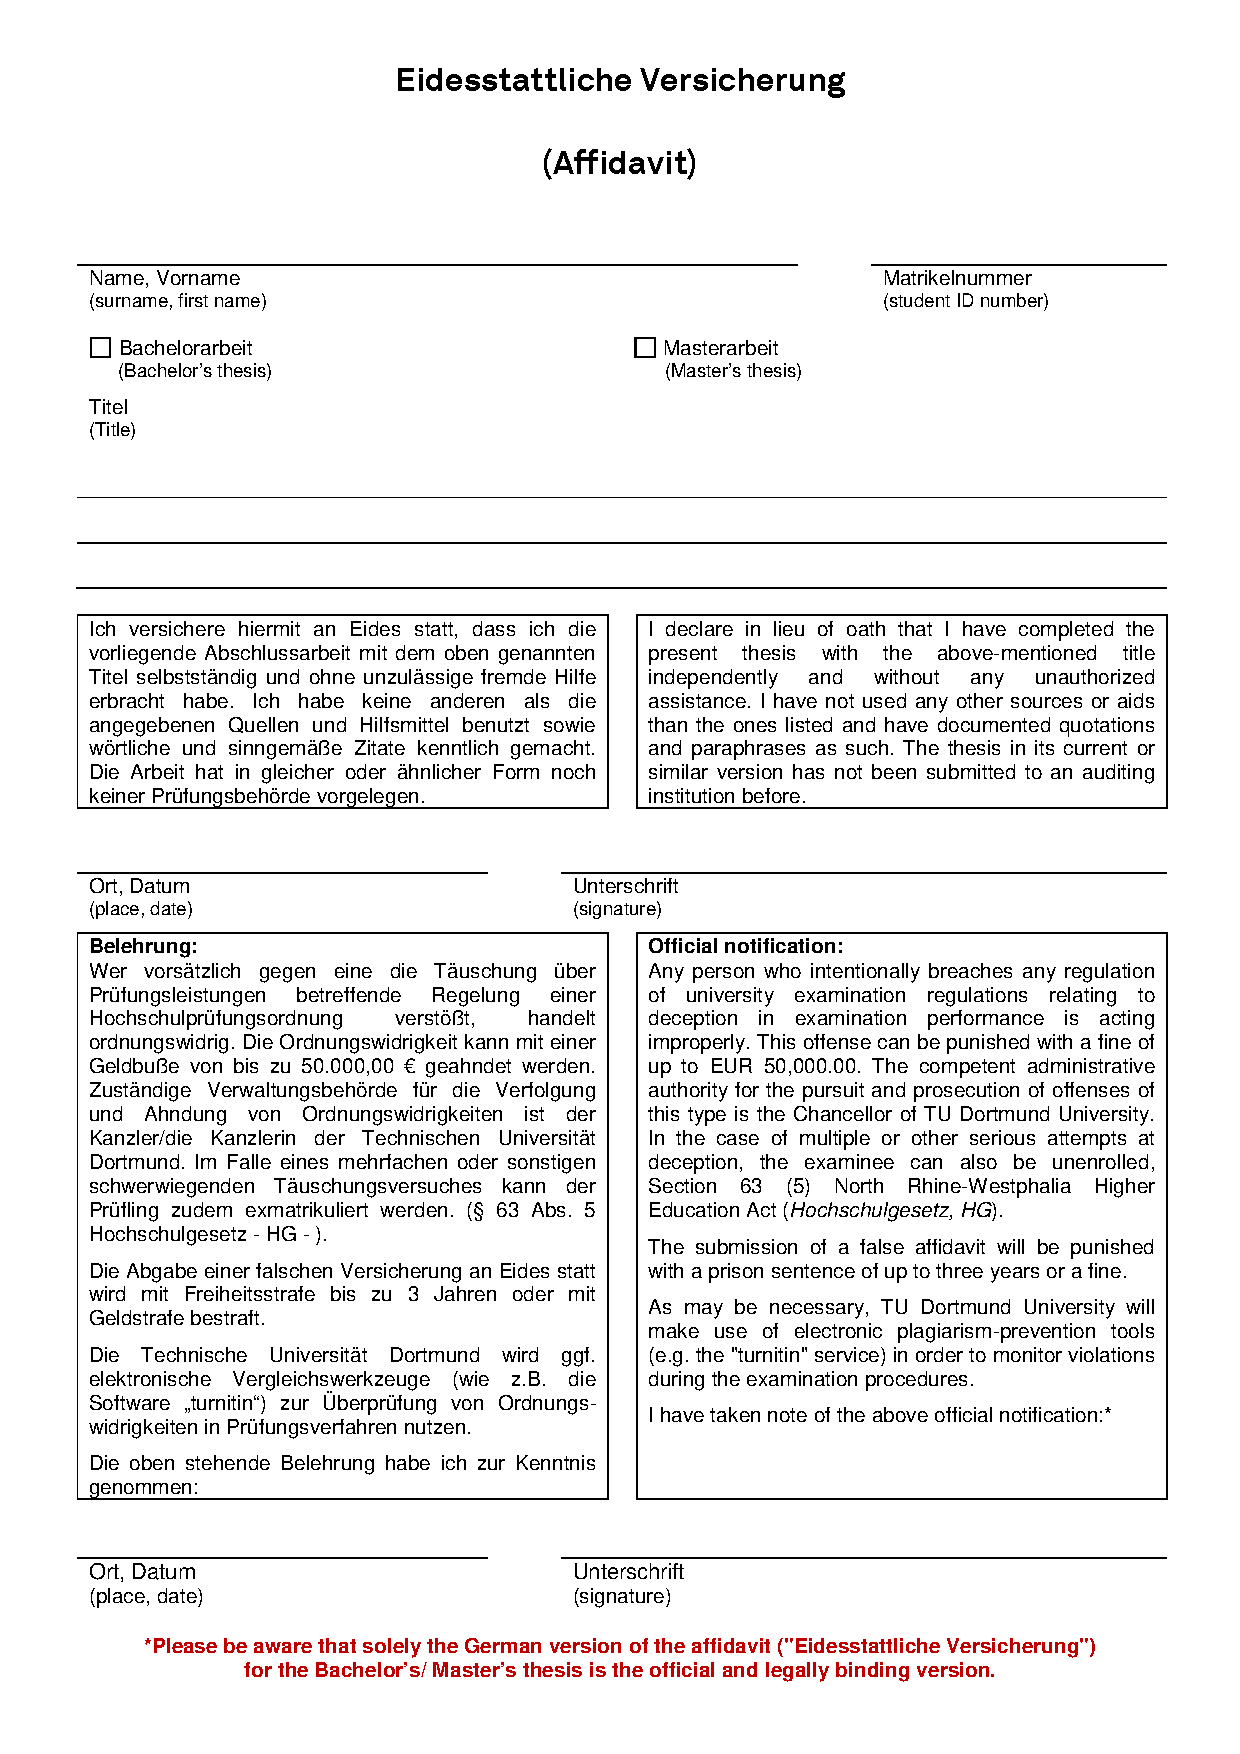
\includepdf{content/Eidesstattliche_Versicherung.pdf}

\end{document}
